\documentclass{article}

\renewcommand{\abstractname}{Individual Assignment 1}

% Set page size and margins
% Replace `letterpaper' with`a4paper' for UK/EU standard size
\usepackage[a4paper,top=1.5cm,bottom=1.5cm,left=2cm,right=2cm,marginparwidth=1cm]{geometry}

% Useful packages
\usepackage{amsmath}
\usepackage{graphicx}
\usepackage[colorlinks=true, allcolors=blue]{hyperref}
\usepackage[tbtags]{amsmath} % for math
\usepackage{minted}

\title{BAM - AS\&P}
\author{Aleksander Odziemkowski}

\begin{document}
\maketitle

\begin{abstract}
\centering
\end{abstract}

\section{Business problem delineation and data preparation}

\subsection{Description of the business problem}

The following document aims at providing relevant stakeholders with a tool to determine house prices in US in a certain market utilizing a linear regression model. Arriving at a certain ask or bid price for a house can be a tedious exercise as many characteristics of the property might be pertinent in a pricing process. Both supply (home-sellers) and demand (home-buyers) in the housing market are in need of a relevant and robust mechanism for the pricing process. The model presented below is meant to solve that problem.

\subsection{Dataset used in the model}

This document makes use of a training set from a \href{https://www.kaggle.com/c/home-data-for-ml-course/data?select=train.csv}{Kaggle competition}. The data set consists of 1,460 observations of residential homes in \href{https://www.google.com/maps/place/Ames,+IA,+USA/@42.0258192,-93.6964165,12z/data=!4m13!1m7!3m6!1s0x87ee70624634a06b:0x273156083cc75200!2sAmes,+IA,+USA!3b1!8m2!3d42.0307812!4d-93.6319131!3m4!1s0x87ee70624634a06b:0x273156083cc75200!8m2!3d42.0307812!4d-93.6319131}{Ames, Iowa} described by their sale price and 79 other variables. 

The analyses that will follow attempt to retrieve variables that best explain the arrival on the transaction price of a house given the dataset and given the theoretical model in the \hyperref[sec:theory]{Section 2}. \emph{SalePrice} is being regressed on the following explanatory variables: \emph{LotArea, LotShape, GarageArea} and \emph{OverallQual}. Among the characteristics being modelled are both numerical variables (\emph{SalePrice}, \emph{LotArea}, \emph{GarageArea}) and categorical variables on an ordinal (\emph{OverallQual}) and nominal (\emph{LotShape}) level of measurement. \emph{LotShape} is being treated as a dummy variable, where 1 represents a regularly shaped lot and 0 corresponds to the irregular shape. \emph{OverallQual} is being enriched in terms of level of measurement and treated as numerical. Reasons for aforementioned treatments are discussed in \hyperref[sec:theory]{Section 2}. Below are the summary statistics of the variables of choice from the dataset:

\begin{table}[!htbp]
\centering
\caption{\label{tab:descriptive} Summary statistics of the variables of choice.}
\begin{tabular}{@{\extracolsep{5pt}}lccccccc} 
\\[-1.8ex]\hline 
\hline \\[-1.8ex] 
Statistic & \multicolumn{1}{c}{Mean} & \multicolumn{1}{c}{St. Dev.} & \multicolumn{1}{c}{Min} & \multicolumn{1}{c}{Pctl(25)} & \multicolumn{1}{c}{Median} & \multicolumn{1}{c}{Pctl(75)} & \multicolumn{1}{c}{Max} \\ 
\hline \\[-1.8ex] 
SalePrice & 180,921.20 & 79,442.50 & 34,900 & 129,975 & 163,000 & 214,000 & 755,000 \\ 
LotArea & 10,516.83 & 9,981.26 & 1,300 & 7,553.5 & 9,478.5 & 11,601.5 & 215,245 \\ 
GarageArea & 472.98 & 213.80 & 0 & 334.5 & 480 & 576 & 1,418 \\ 
OverallQual & 6.10 & 1.38 & 1 & 5 & 6 & 7 & 10 \\ 
dLotShapeRegular & 0.63 & 0.48 & 0 & 0 & 1 & 1 & 1 \\ 
\hline \\[-1.8ex] 
\end{tabular} 
\end{table} 

Each variable has a complete set of 1,460 instances. Presentation of quartiles gives an initial sense of the distribution of the data. For categorical variables it can be derived that there is more houses with better than average overall material and finish of the house and more regularly shaped lots. Worth noting is a wide range of values for numerical variables: \emph{SalePrice}(1,300; 215,245), \emph{LotArea}(1,300; 215,245), \emph{GarageArea}(0; 1,418).
Calculation of coefficient of variance (defined as the ratio of the standard deviation to the mean) of the data above suggests that the data is quite dispersed for \emph{LotArea} (94.91\%) and \emph{LotShape} (76.08\%). For other variables in the consideration CV is below 50\%.

\subsection{Data visualization}

Below are the graphs which contribute to the theoretical model that will be discussed in the following section by plotting explanatory variables against the explained one. 

\hyperref[fig:LotArea]{Figure 1} shows that the positive relationship can be observed between \emph{LotArea} and \emph{SalePrice} where the overall dependence seems to be of a very steep nature. Additionally, \emph{LotArea} is grouped by \emph{LotShape}, where regularly shaped lots appear to have a stronger positive association with \emph{SalePrice} than irregularly shaped lots of different degree.  

\begin{figure}[htp]
    \caption{Relationship between \emph{LotArea} ($m^{2}$) and \emph{SalePrice} (\$) with regards to the lot shape.}
    \centering
    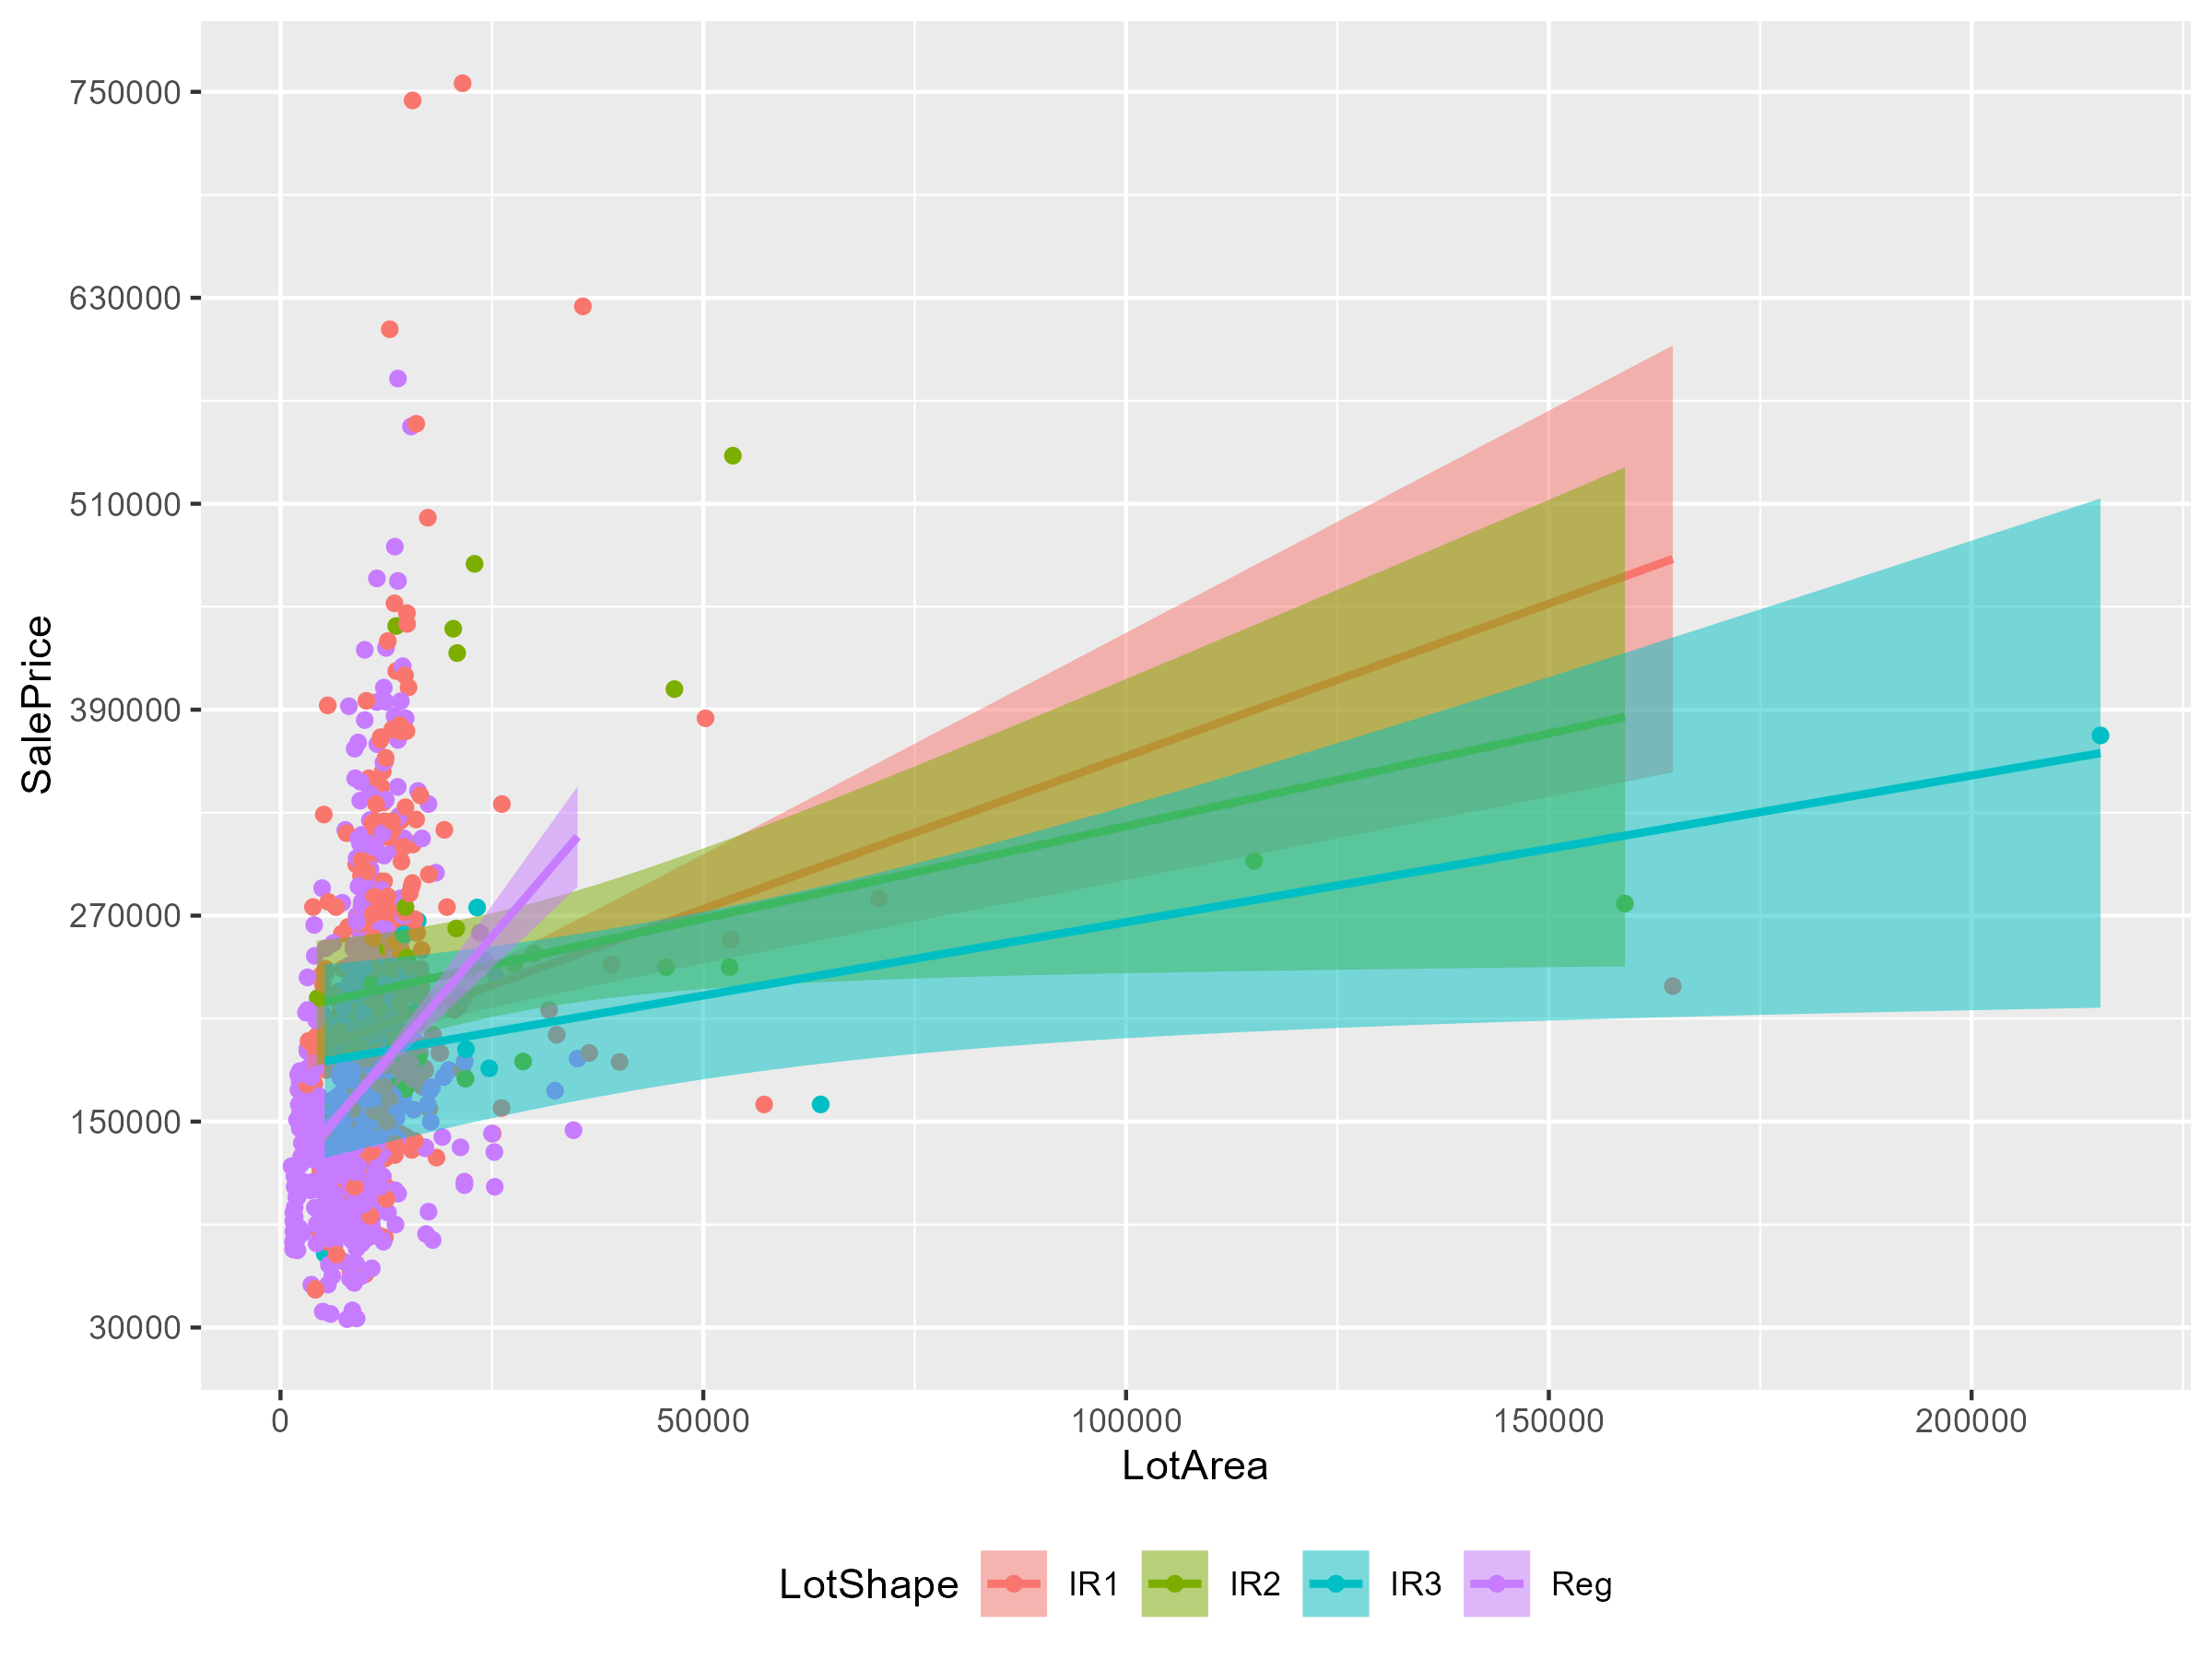
\includegraphics[width=0.55\textwidth]{scatterLotShapeInteraction}
    \label{fig:LotArea}
\end{figure}

\hyperref[fig:dLotShapeRegular]{Figure 2} illustrates the proportion of different categories used in a dataset for \emph{LotShape}. Left-hand side y-axis counts the instances of each category of lot shape whilst right-hand side y-axis reflects those frequencies in relation to the total number of observations. Regularly shaped lots amount to 63\% of 1,460 observations. The other 37\% comprises of three categories of irregularly shaped lots. However, categories \emph{IR2} and \emph{IR3} add up to only 3.5\% of observations so for the purpose of turning \emph{LotShape} into a dummy variable all irregular shapes (\emph{IR1, IR2, IR3}) are aggregated into a single category as it will not result in losing significant amount of information. In the model this aggregation is presented under variable \emph{dLotShapeRegular}. 

\begin{figure}[htp]
    \caption{Absolute and relative frequencies of categories of lot shapes in the dataset.}
    \centering
    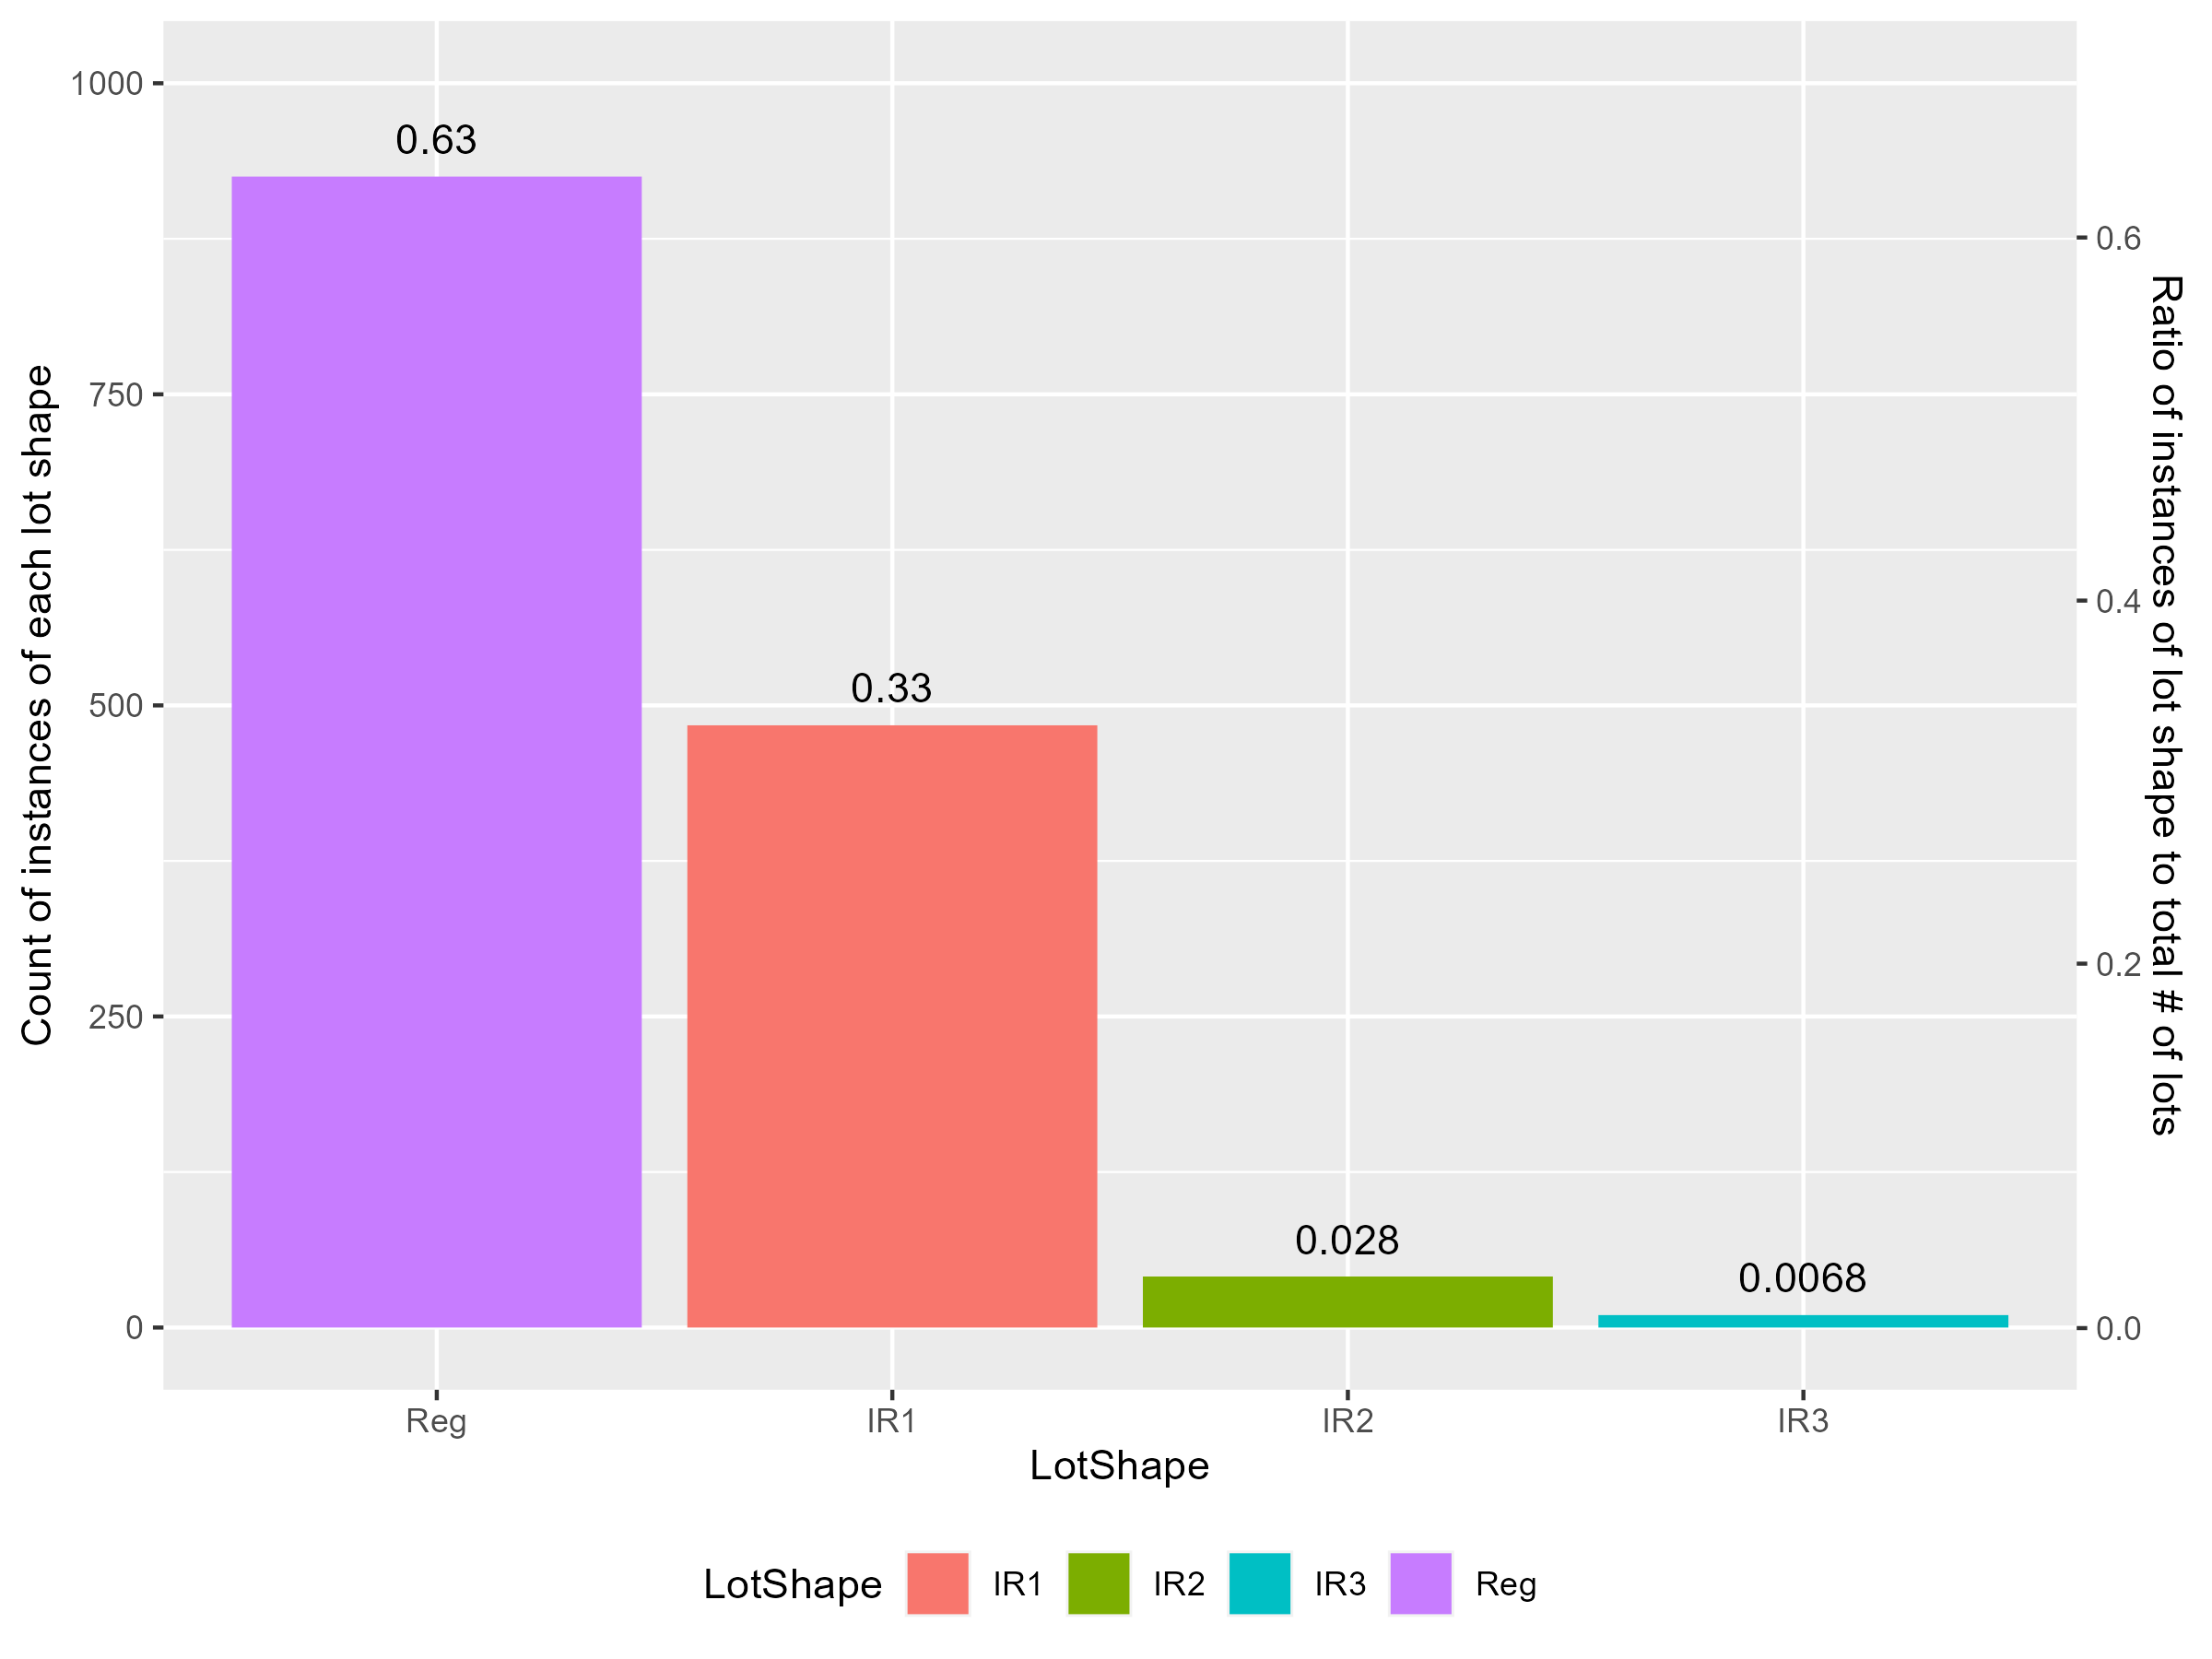
\includegraphics[width=0.55\textwidth]{barBaseShapeAggregate}
    \label{fig:dLotShapeRegular}
\end{figure}

Furthermore, the reason for treatment of a categorical variable \emph{OverallQual} as numerical is being depicted in \hyperref[fig:scatterBaseQualityLinear]{Figure 3}. 

\begin{figure}[htp]
    \caption{Relationship between \emph{OverallQual} and \emph{SalePrice} (\$).}
    \centering
    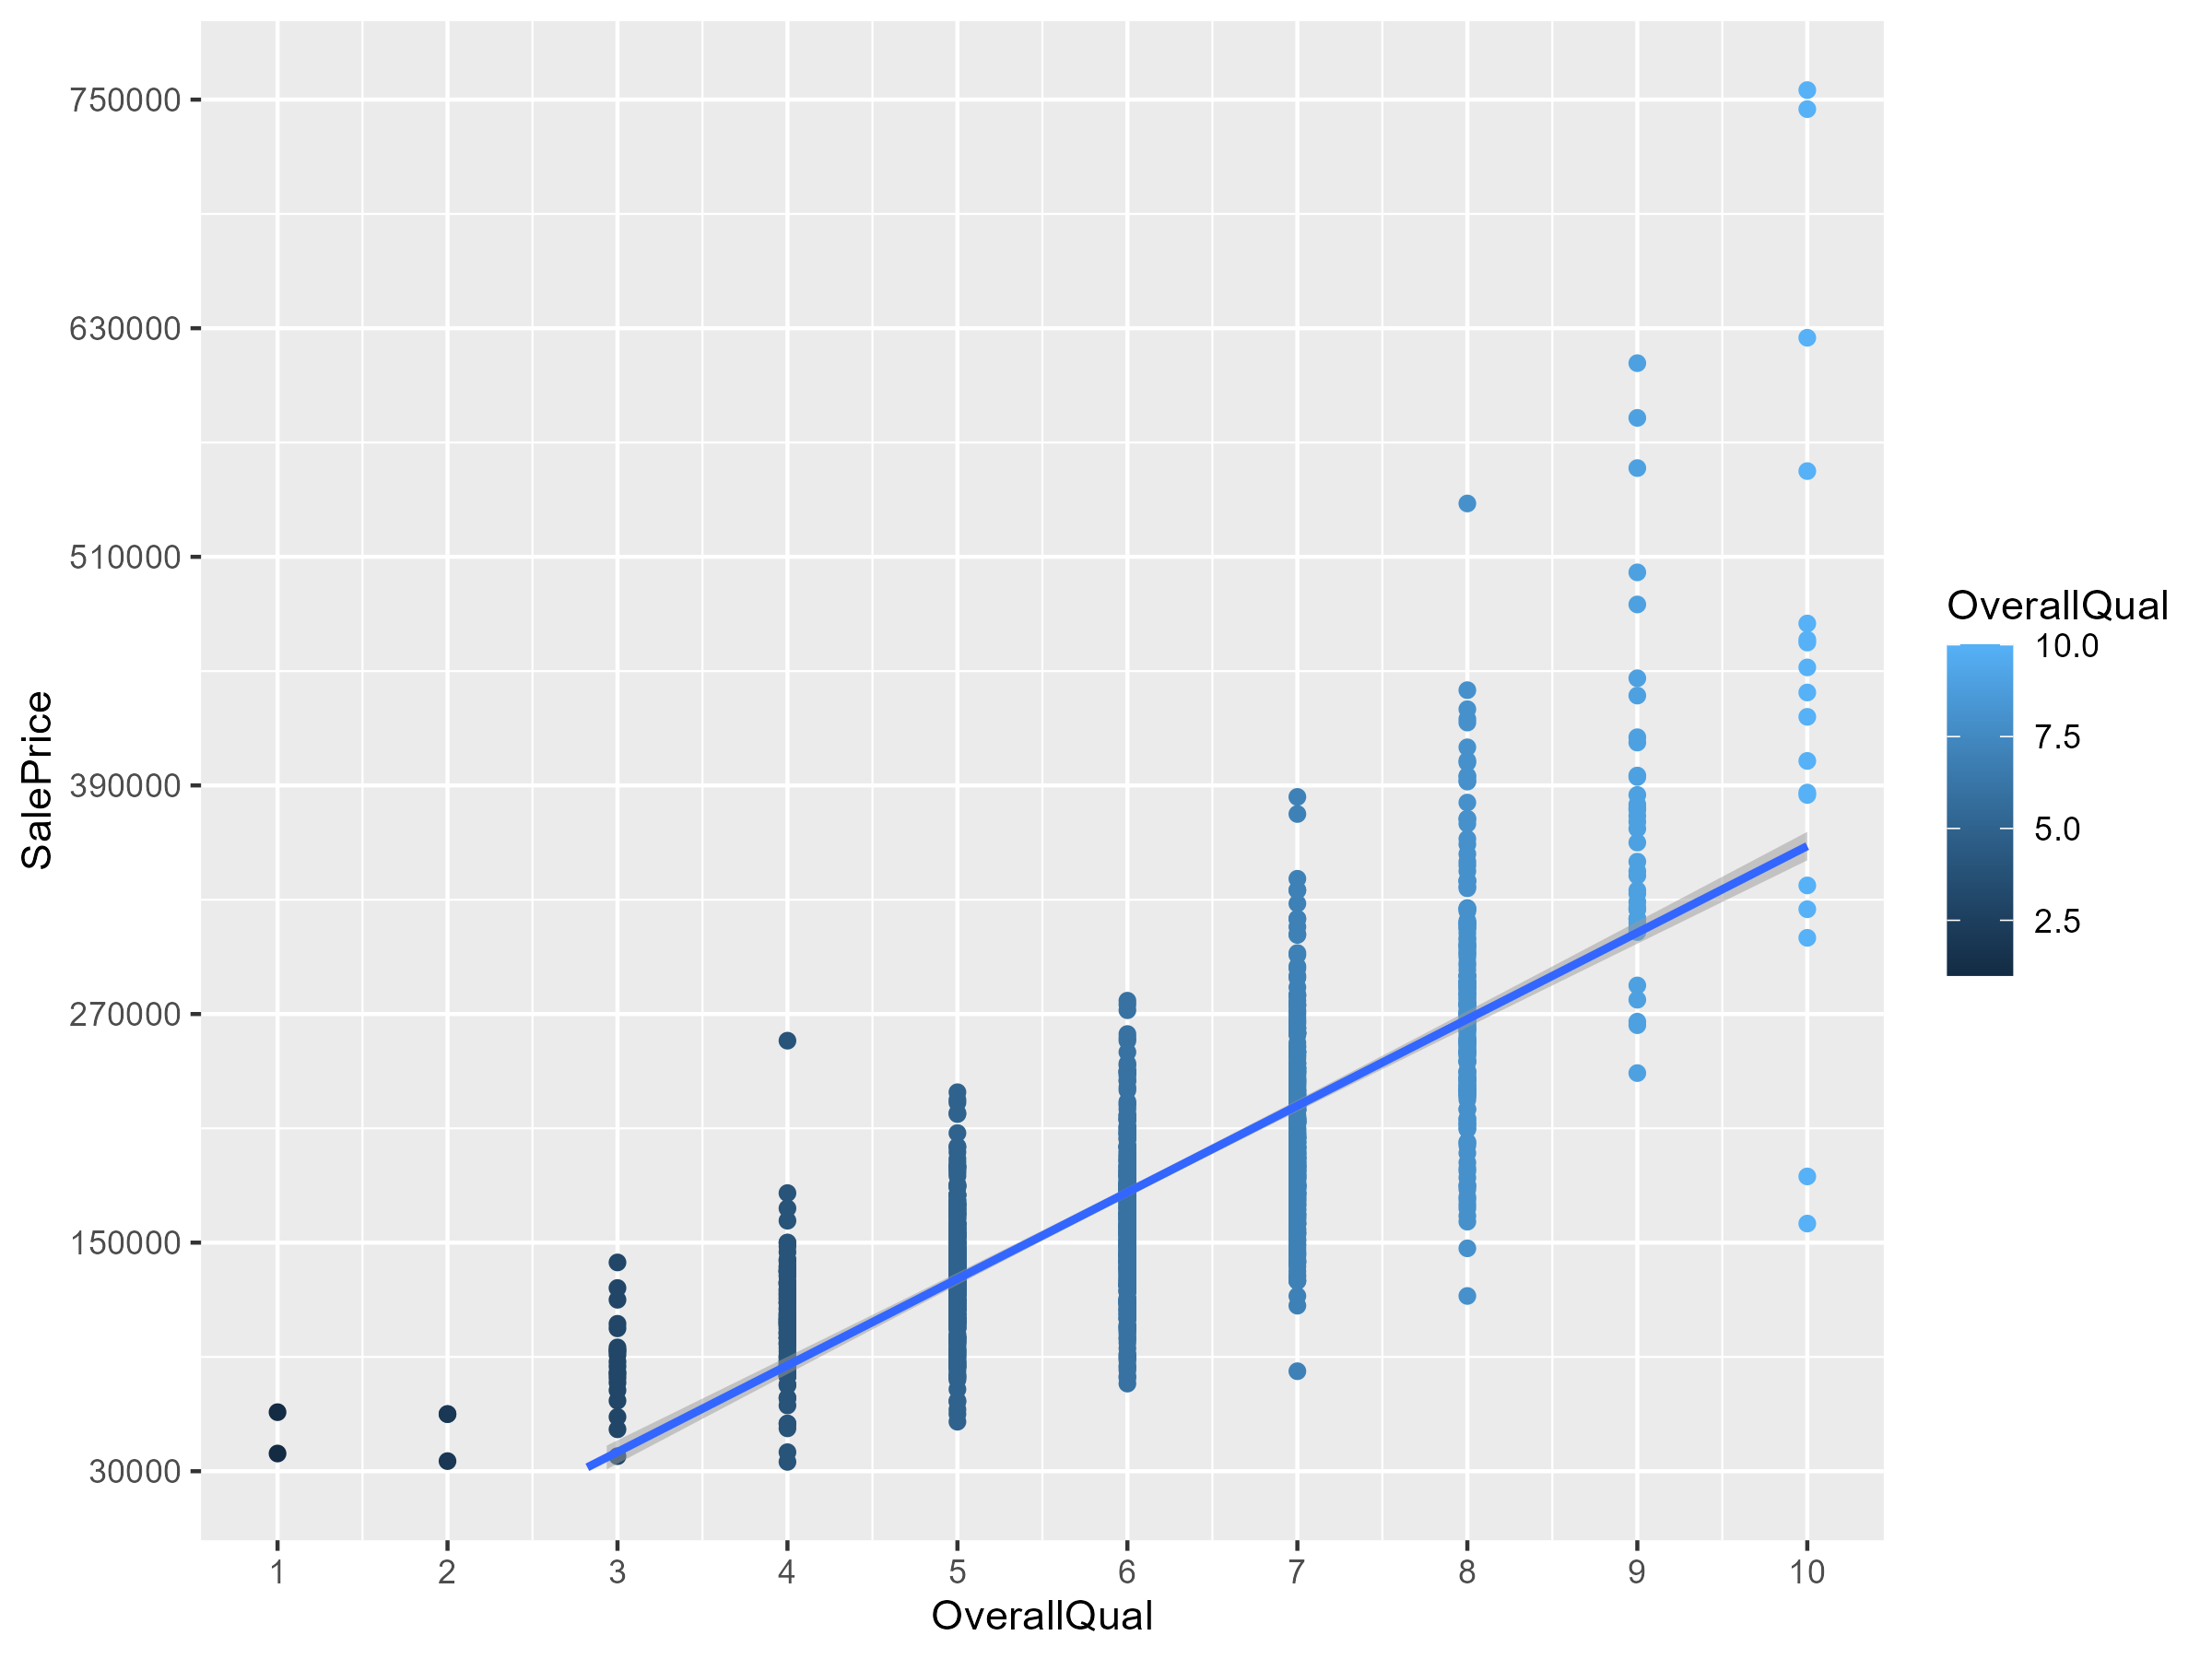
\includegraphics[width=0.55\textwidth]{scatterBaseQualityLinear}
    \label{fig:scatterBaseQualityLinear}
\end{figure}

What initially was a scale of 1-10 will now be considered directly as a quantitative measure due to the linear relationship of effects of consecutive increases in quality on \emph{SalePrice}. 

This assumption is drawn from the fitted line in \hyperref[fig:scatterBaseQualityLinear]{Figure 3} as well as by looking at the trend of linearly increasing coefficients in a table in \hyperref[tab:overallqualldummy]{Appendix A}. The direct interpretation of beta associated with \emph{OverallQual} will have no precise meaning, but the general association and standardized strength of the effect can now be measured and interpreted more easily. 

\section{Theoretical model and OLS assumptions}
\label{sec:theory}

\subsection{Causal relationship diagram and the theory behind the model}

A theoretical aspect of the model that allows for an estimation of a data generating process of \emph{SalePrice} given a chosen set of explanatory variables can be derived from a \hyperref[fig:causaldiagram]{causal diagram} below. The primary goal of such graph is to represent
explicitly all associations in the model based on assumptions grounded in the theory. 

\begin{figure}[htp]
    \caption{Causal diagram based on the theory behind the model.}
    \centering
    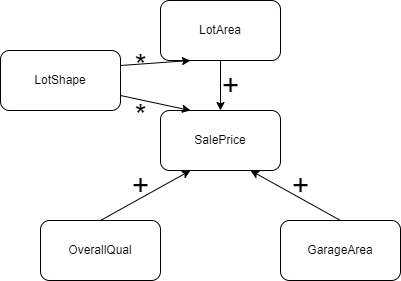
\includegraphics[width=0.4\textwidth]{causal_diagram}
    \label{fig:causaldiagram}
\end{figure}

A theory behind the model is as follows. Variation in values of \emph{SalePrice} can be explained by the overall material and finish of the house because the better the foundations and building blocks of the construction the higher the price will buyers bid (sellers ask) for the property. Moreover, the bigger the area of the lot being priced, the more footage is there to be priced in, so the \emph{SalePrice} will be higher. 

Given the underlying region of the dataset, \emph{GarageArea} plays a big part in the valuation of the house. In the case of remote flat plains and gently rolling hills of Iowa, US, home-owners highly value owning a car (or multiple cars) and consequently - their garage space. It is a factor that should be positively associated with the price of the house. Additionally, due to restrictions on potential floor plans and general use case for home-owners, irregularly shape lots tend to be harder to sell. Hence, they end up being bid or asked lower than regularly shaped properties. These assumptions are reflected in \hyperref[fig:causaldiagram]{Figure 4}.

\subsection{Research hypotheses and population regression model}
\label{sec:hypotheses}
This document reflects on the following three research hypotheses that are being examined in \hyperref[sec:olsfit]{Section 3}.

H\textsubscript{1}: Garage area has a positive influence on the sale price of the house.

H\textsubscript{2}: The expected sale price of the house is higher for houses with a better overall material and finish of the house.

H\textsubscript{3}: The positive influence of lot size on sale price of the house is expected to be larger for regularly shaped lots than for irregularly shaped ones.

The following part will introduce several regression models for the population. Population regression model without any specifications:
\begin{gather}
SalePrice=\ \beta_0\ +\ \beta_1LotArea\ +\ \beta_2GarageArea\ +\ \beta_3LotShape\ +\ \\ \beta_4OverallQual\ +\ \varepsilon,\ \ \varepsilon\ ~\ n(0,\ \sigma)
\end{gather}

Population regression model introducing a non-linear term:
\begin{gather}
SalePrice=\ \beta_0\ +\ \beta_1LotArea\ +\ \beta_2GarageArea\ +\ \beta_3LotShape\ +\ \beta_4OverallQual\ +\ \\ 
\beta_5LotArea2\ +\ \varepsilon,\ \ \varepsilon\ ~\ n(0,\ \sigma)
\end{gather}

The quadratic term is introduced for \emph{LotArea} because $R^{2}$ improvement and meaningful change in coefficients suggest that introducing quadratic terms for LotArea instead of \emph{GarageArea} will be more beneficial for the model. A short summary on simple regression models used as a decision rule is provided in the Appendix A \hyperref[tab:quadraticlotarea]{here} and \hyperref[tab:quadraticgaragearea]{here}.

Population regression model introducing dummy variable specification:
\begin{gather}
SalePrice=\ \beta_0\ +\ \beta_1LotArea\ +\ \beta_2GarageArea\ +\ \beta_3dLotShapeRegular\ +\ \\ \beta_4OverallQual\ +\ \varepsilon,\ \ \varepsilon\ ~\ n(0,\ \sigma) 
\end{gather}

Population regression model introducing interactions:
\begin{gather}
SalePrice=\ \beta_0\ +\ (\beta_{11}+\beta_{12}dLotShapeRegular)LotArea\ +\ \beta_2GarageArea\ +\ \\ \beta_3dLotShapeRegular\ +\
\beta_4OverallQual\ \ +\ \varepsilon,\ \ \varepsilon\ ~\ n(0,\ \sigma)
\end{gather}

\subsection{Possible violations of the assumptions}

The assumption of linearity of the regression model (A1) specifies a linear relationship between explanatory variables and the regressand while also accounting for additive disturbances. The violation of A1 might occur if the underlying function by which parameters beta enter the model is nonlinear.

Second assumption pertains to the full rank of column space for explanatory variables (A2). Basically, there should be no exact linear relationship among any of the independent variables in the model. For the dataset considered in this document, a violation could occur if, for example, \emph{GarageArea} would be generated directly from \emph{LotArea} by taking an arbitrary percent and deriving it from the latter variable to arrive at the former. 

A third assumption is related to the exogeneity of independent variables - the expected value of a disturbance at any observation in the sample should not be related functionally to the independent variables observed at that certain observation (A3). Violation is prone to occur if variables highly correlated with explanatory terms are excluded from the model and consequently contaminate disturbances with entangled correlations.

Homoscedasticity (constant variance of disturbances) is the fourth assumption (A4). Violation of A4 would occur in an instance where there is a systematic change in the spread of the residuals over the range of measured values - an example would be an increasing variance of \emph{SalePrice} as the \emph{LotSize} increases which might have been caused by, for example, a difference in the long-term maintenance of evaluated lots.

Assumption A5 is about a data generating process under which regressors are assumed to be fixed or random. In a data considered in this document, the variables are not under control (observed but not set). Violation could occur if, for example, an adverse shock to economic cycles is applied and macroeconomic conditions for the housing markets change whilst our model based on a fixed dataset does not respond to said shock. 

Assumption A6 assumes normality of disturbances. If A6 is violated, then the results of model's hypothesis tests and confidence intervals for \emph{SalePrice} are inaccurate and might be perceived as less useful by the stakeholders.

\section{OLS regression and model fit}
\label{sec:olsfit}
\subsection{Sample regression models}

Given the population regression models defined in \hyperref[sec:hypotheses]{Subsection 2.2} this section will present and examine the estimation results of 4 sample regression models.

\begin{table}[h]
\centering
\caption{\label{tab:sampleregression} Sample regression models (1) without specifications and after introducing (2) interaction and (3) quadratic term.}
\begin{tabular}{@{\extracolsep{5pt}}lccc} 
\\[-1.8ex]\hline 
\hline \\[-1.8ex] 
 & \multicolumn{3}{c}{\textit{Dependent variable:}} \\ 
\cline{2-4} 
\\[-1.8ex] & \multicolumn{3}{c}{SalePrice} \\ 
\\[-1.8ex] & (1) & (2) & (3)\\ 
\hline \\[-1.8ex] 
 LotArea & 1.112$^{***}$ & 0.940$^{***}$ & 2.748$^{***}$ \\ 
  & (0.118) & (0.123) & (0.264) \\ 
  & & & \\ 
 I(LotArea$\hat{\mkern6mu}$2) &  &  & $-$0.00001$^{***}$ \\ 
  &  &  & (0.00000) \\ 
  & & & \\ 
 GarageArea & 85.709$^{***}$ & 78.641$^{***}$ & 76.251$^{***}$ \\ 
  & (6.527) & (6.640) & (6.569) \\ 
  & & & \\ 
 dLotShapeRegular1 & $-$11,916.440$^{***}$ & $-$30,155.460$^{***}$ & $-$8,720.940$^{***}$ \\ 
  & (2,467.157) & (4,495.212) & (2,471.974) \\ 
  & & & \\ 
 OverallQual & 36,311.880$^{***}$ & 36,584.710$^{***}$ & 36,444.000$^{***}$ \\ 
  & (1,005.548) & (999.486) & (989.935) \\ 
  & & & \\ 
 LotArea:dLotShapeRegular1 &  & 1.925$^{***}$ &  \\ 
  &  & (0.398) &  \\ 
  & & & \\ 
 Constant & $-$85,240.480$^{***}$ & $-$81,022.080$^{***}$ & $-$98,493.990$^{***}$ \\ 
  & (5,891.708) & (5,911.517) & (6,107.664) \\ 
  & & & \\ 
\hline \\[-1.8ex] 
Observations & 1,460 & 1,460 & 1,460 \\ 
R$^{2}$ & 0.700 & 0.705 & 0.710 \\ 
Adjusted R$^{2}$ & 0.699 & 0.704 & 0.709 \\ 
Residual Std. Error & 43,569.400 (df = 1455) & 43,237.750 (df = 1454) & 42,884.910 (df = 1454) \\ 
F Statistic & 848.907$^{***}$ (df = 4; 1455) & 694.265$^{***}$ (df = 5; 1454) & 710.541$^{***}$ (df = 5; 1454) \\ 
\hline 
\hline \\[-1.8ex] 
\textit{Note:}  & \multicolumn{3}{r}{$^{*}$p$<$0.1; $^{**}$p$<$0.05; $^{***}$p$<$0.01} \\ 
\end{tabular} 
\end{table} 

\hyperref[tab:sampleregression]{Table 2} estimates the results of sample regression models for instances without any specifications, as well as for interaction and quadratic term (separately). 

For every model in \hyperref[tab:sampleregression]{Table 3}, all explanatory variables yield positive significant results (in terms of p-value < 0.01). 

In model (1), the size of the lot as well as the garage area can significantly differentiate a price of the house - with a squared meter increase in a garage size, the price for the property increases by \$85.71, whilst an additional squared meter of the lot area is estimated to result in an increase of \emph{SalePrice} by \$1.11. Coefficient for \emph{OverallQual} informs about higher price of house that is finished with higher quality materials in comparison to those with worse quality. The estimate of the effect for shape of the lot gives information about a decrease of the \emph{SalePrice} by \$11,916.44 if the lot is shaped regularly. 

Model (2) can be assessed in terms of the interaction effect of lot shape on the lot area which is of interest in the light of research hypotheses. For lots shaped irregularly, change in unit of lot area corresponds with a \$.94 increase in the price of the house. However, if the house is shaped regularly, the interaction effect increases the change of lot area's impact on the \emph{SalePrice} to \$2.87. All in all, regular shape of lot contributes to the increase of the sale price stronger than the irregular one.

Although introduction of quadratic term in the model (3) enlarges the magnitude of the positive association between \emph{LotArea} and \emph{SalePrice} by \$1.64, this change can hardly be explained by the impact of quadratic term effect (negative effect of 0.00001).

All three models exhibit rather high explanatory power; over 70\%
of variation in \emph{SalePrice} has been explained (F statistics significant at p < 0.01). It is worth noting that a model fit slightly improves with an introduction of the interaction effect \emph{LotArea:dLotShapeRegular}; the fit is upgraded even more by the introduction of quadratic term on \emph{LotArea}.  

The results presented in the \hyperref[tab:sampleregressionall]{table in the Appendix A} refer to an estimation of sample regression model with quadratic term and an interaction jointly. Overall, worth noting is that introducing  additional specifications increases the effect size on the dependent of \emph{LotArea} whereas the other coefficients are relatively unchanged.

\subsection{Standardized effects}

Estimated coefficients have a certain dimension. Unit of measurements of parameters depends on the ratio of the unit of measurement of the dependent variable and the corresponding independent variable. Difference in dimensions of measurement can create issues with interpreting the strength of an effect. 

\begin{table}[h]
\centering
\caption{\label{tab:standardizedeffects} Standardized effects for each of four sample regression models.}
\begin{tabular}{l|r|r|r|r}
\hline
  & Baseline & Interactions & Non-linear & Interactions and non-linear\\
\hline
(Intercept) & \emph{NA} & \emph{NA} & \emph{NA} & \emph{NA}\\
\hline
dLotShapeRegular1 & -0.0723 & -0.1830 & -0.0529 & -0.0948\\
\hline
GarageArea & 0.2307 & 0.2116 & 0.2052 & 0.2018\\
\hline
I(LotArea\textasciicircum{}2) & \emph{NA} & \emph{NA} & -0.2223 & -0.1931\\
\hline
LotArea & 0.1397 & 0.1181 & 0.3453 & 0.3106\\
\hline
LotArea:dLotShapeRegular1 & \emph{NA} & 0.1278 & \emph{NA} & 0.0454\\
\hline
OverallQual & 0.6321 & 0.6369 & 0.6344 & 0.6358\\
\hline
\end{tabular}
\end{table} 

To mitigate this issue and present a unified metric for assessing the size of the effect of explanatory variables on the dependent variable standardized effects are computed and compared in \hyperref[tab:standardizedeffects]{Table 3}. 

It can be assessed that across all sample regression models it is \emph{OverallQual} that has the largest effect size on the dependent variables amongst all explanatory variables. As no specifications are introduced to this variable directly, the effect size is rather constant for every model - around 0.63. The same can be said about constancy of the \emph{GarageArea} effect at a level of around 0.20 to 0.23. For \emph{LotArea} it seems that introducing quadratic term does not affect the effect size much in comparison to baseline model, whilst when interacting with the \emph{dLotShapeRegular} the effect size of area of the lot for regularly shaped lots largely increases (0.1181 + 0.1278).

\section{Diagnostic analysis}

The following section will systematically analyze if model assumptions have been violated for the estimated model with interaction and non-linear term. 

\subsection{Full rank and multicollinearity}

Assumption A2 discusses the issue of having a perfect linear dependence between explanatory variables in the dataset. This issue might happen, but rather rarely and is not existent in this model. However, worth investigating is the data issue of multicollinearity, so an almost exact linear relationship of the coviarates. In such case interpretation of the model and its fit is damaged.

\begin{figure}[htp]
    \caption{Correlation matrix for the baseline model.}
    \centering
    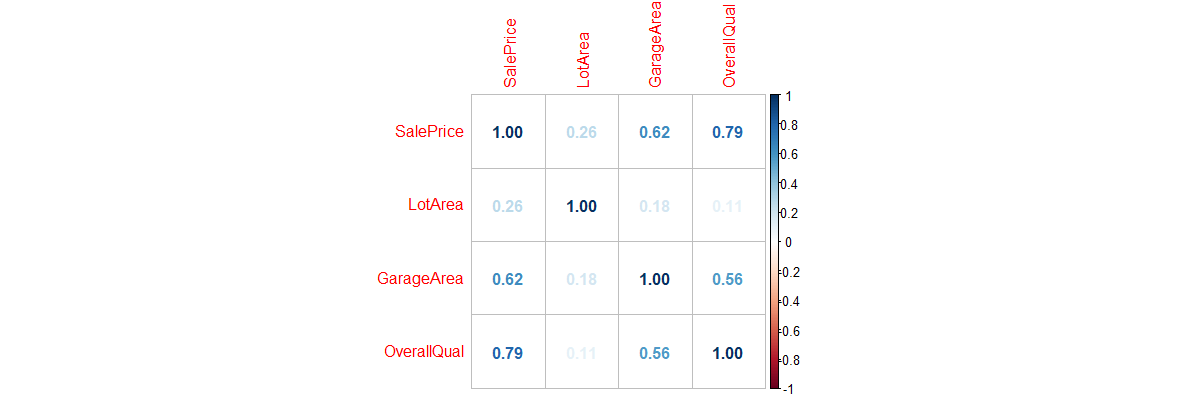
\includegraphics[width=0.6\textwidth]{corrplot.png}
    \label{fig:correlationmatrix}
\end{figure}

Multicollinearity happens when independent variables are highly correlated to each other. Firstly, the \hyperref[fig:correlationmatrix]{correlation matrix} is presented. None of the variables reach a very strong (say over 0.80) correlation given by Pearson's correlation coefficient. Nonetheless, \emph{OverallQual} has a highest value of the correlation measure with 0.79. Subsequently, multicollinearity is investigated using VIF indicator.

\begin{table}[!htbp]
\centering
\caption{\label{tab:vif} VIF indicator for baseline model.}
\begin{tabular}{@{\extracolsep{5pt}} cccc} 
\\[-1.8ex]\hline 
\hline \\[-1.8ex] 
LotArea & GarageArea & dLotShapeRegular & OverallQual \\ 
\hline \\[-1.8ex] 
$1.073$ & $1.497$ & $1.087$ & $1.486$ \\ 
\hline \\[-1.8ex] 
\end{tabular} 
\end{table}

\hyperref[tab:vif]{Table 5} indicates that none of the explanatory variables exceed an arbitrary threshold for VIF indicator (usually at 5.0) that would suggest an existence of multicollinearity in the model. Thus, it can be concluded that such data issue is not in play.

\subsection{Normality of error terms}

In the regression model, A6 implies that variation in the disturbances in the model is not explained by variation in the independent variables. Consequently, those disturbances should be statistically independent of each other. The assumption can be tested by looking at the graphical evidence for residuals and Studentized residuals.

If the assumption of OLS holds, the empirical 0 should be the mean. Moreover, looking at the range(min;max), similar magnitude on both ends should be observed to reflect normal distribution.

\begin{table}[!htbp]
\centering
\caption{\label{tab:residuals} Summary statistics for residuals of all models.}
\begin{tabular}{@{\extracolsep{5pt}}lccccc} 
\\[-1.8ex]\hline 
\hline \\[-1.8ex] 
Statistic & \multicolumn{1}{c}{N} & \multicolumn{1}{c}{Mean} & \multicolumn{1}{c}{St. Dev.} & \multicolumn{1}{c}{Min} & \multicolumn{1}{c}{Max} \\ 
\hline \\[-1.8ex] 
resids\_baseline & 1,460 & 0.000 & 43,509.640 & $-$310,459.400 & 381,863.800 \\ 
resids\_interactions & 1,460 & $-$0.000 & 43,163.600 & $-$296,374.000 & 384,508.900 \\ 
resids\_nonlinear & 1,460 & $-$0.000 & 42,811.370 & $-$344,790.500 & 376,810.800 \\ 
resids\_interactions\_nonlinear & 1,460 & $-$0.000 & 42,779.240 & $-$335,281.300 & 377,768.100 \\ 
studresids\_baseline & 1,460 & 0.0002 & 1.008 & $-$7.362 & 9.035 \\ 
studresids\_interactions & 1,460 & 0.0002 & 1.008 & $-$7.089 & 9.176 \\ 
studresids\_nonlinear & 1,460 & 0.001 & 1.011 & $-$8.410 & 9.058 \\ 
studresids\_interactions\_nonlinear & 1,460 & 0.001 & 1.012 & $-$8.274 & 9.088 \\ 
\hline \\[-1.8ex] 
\end{tabular} 
\end{table}

Results in \hyperref[tab:residuals]{Table 6} highlight that Studentized residuals, which are more conservative by including each residual's standard deviation in the calculations, point in direction of the A6 violation as the mean is not precisely equal to 0, though it is very close. It is worth looking at the graphical evidence which follows.

\begin{figure}[htp]
    \caption{Residuals vs. Fitted for error terms of each of four models.}
    \centering
    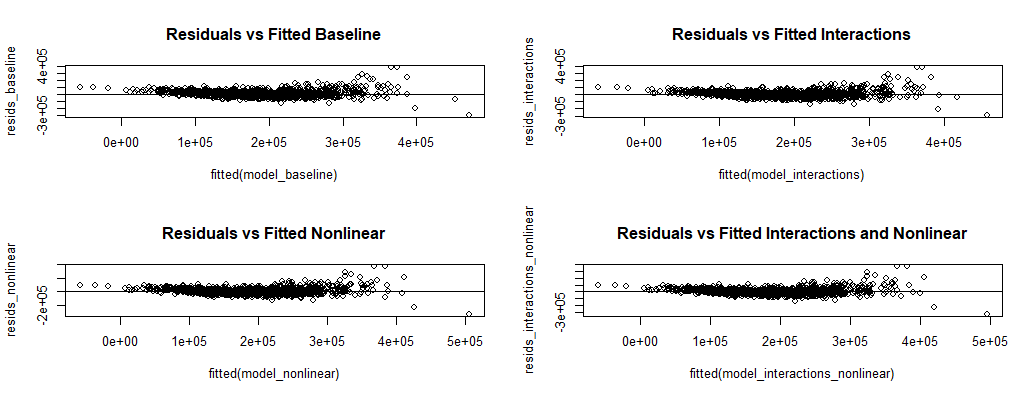
\includegraphics[width=0.6\textwidth]{residuals_fitted.png}
    \label{fig:residualsfitted}
\end{figure}

In case of both residuals \hyperref[fig:residualsfitted]{Figure 6} and Studentized residuals \hyperref[fig:sturesidualsfitted]{Figure 7} the plots suggest that errors are fairly evenly distributed across the mid-line. Possible cause of slight differentiation of the mean from the 0 are more extreme observations toward the upper-end of quantitative variables (\emph{GarageArea, LotArea} and consequently \emph{SalePrice}.

\begin{figure}[htp]
    \caption{Studentized Residuals vs. Fitted for error terms of each of four models.}
    \centering
    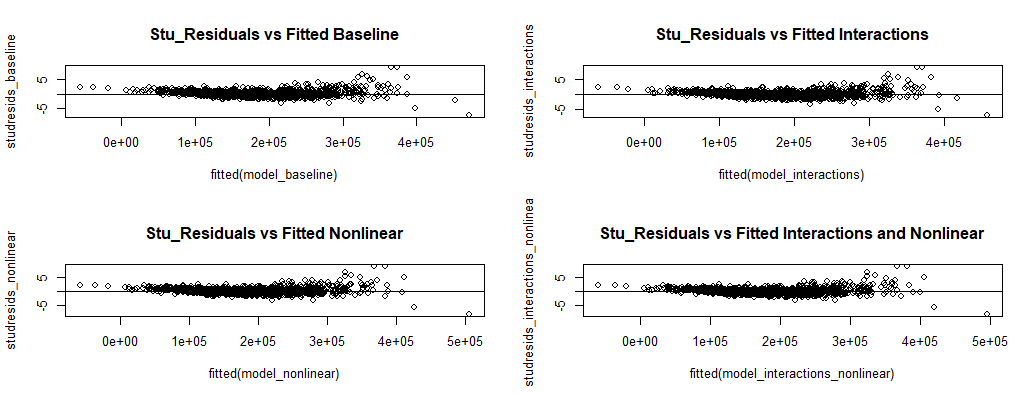
\includegraphics[width=0.4\textwidth]{stu_residuals_fitted.png}
    \label{fig:sturesidualsfitted}
\end{figure}

\subsection{Homoscedasticity}

\begin{figure}[htp]
    \caption{Residuals vs. Fitted in terms of homoscedasticity.}
    \centering
    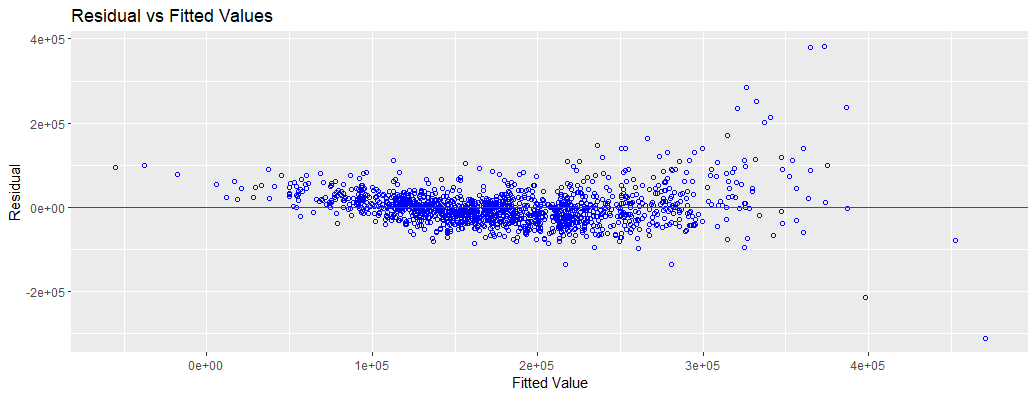
\includegraphics[width=0.5\textwidth]{homoscedasticity.png}
    \label{fig:homoscedasticity}
\end{figure}

Homoscedasticity refers to a constant variance of disturbances in the model. Eventual violation of the assumption can be investigated both graphically and by performing a statistical test. On the Residuals vs. Fitted plot the even distribution of data point around the mid-line confirms the homoscedasticity. \hyperref[fig:homoscedasticity]{Figure 8} can let the observer to believe that in fact the model deals with heteroscedasticity. 

This should be further investigated by performing studentized Breusch-Pagan test. Said test confirms the rejection of the null hypothesis (so suggests existence of heteroscedasticity of error terms with significance) for the baseline model (BP = 125.97, p-value \textless 0.0001).

A remedy for heteroscedasticity of residuals could be an introduction of more robust standard errors. By introducing more conservative approach to the calculations, both White's and clustered standard errors mitigate heteroscedasticity and allow for more confidence in the significance of model's estimates. 

\begin{table}[h]
\centering
\caption{\label{tab:standarderrors} More robust standard errors mitigating heteroscedasticity in the baseline model. (1) basic SE, (2) White's SE, (3) clustered SE on the lot shape.}
\begin{tabular}{@{\extracolsep{5pt}}lccc} 
\\[-1.8ex]\hline 
\hline \\[-1.8ex] 
 & \multicolumn{3}{c}{\textit{Dependent variable:}} \\ 
\cline{2-4} 
\\[-1.8ex] & \multicolumn{3}{c}{SalePrice} \\ 
\\[-1.8ex] & (1) & (2) & (3)\\ 
\hline \\[-1.8ex] 
 LotArea & 1.112$^{***}$ & 1.112$^{***}$ & 1.112$^{***}$ \\ 
  & (0.118) & (0.227) & (0.272) \\ 
  & & & \\ 
 GarageArea & 85.709$^{***}$ & 85.709$^{***}$ & 85.709$^{***}$ \\ 
  & (6.527) & (7.388) & (7.558) \\ 
  & & & \\ 
 dLotShapeRegular0 & 11,916.440$^{***}$ & 11,916.440$^{***}$ & 11,916.440$^{***}$ \\ 
  & (2,467.157) & (2,393.039) & (2,433.623) \\ 
  & & & \\ 
 OverallQual & 36,311.880$^{***}$ & 36,311.880$^{***}$ & 36,311.880$^{***}$ \\ 
  & (1,005.548) & (1,404.749) & (1,415.765) \\ 
  & & & \\ 
 Constant & $-$97,156.920$^{***}$ & $-$97,156.920$^{***}$ & $-$97,156.920$^{***}$ \\ 
  & (5,229.643) & (8,552.239) & (8,685.002) \\ 
  & & & \\ 
\hline \\[-1.8ex] 
Observations & 1,460 & 1,460 & 1,460 \\ 
R$^{2}$ & 0.700 & 0.700 & 0.700 \\ 
Adjusted R$^{2}$ & 0.699 & 0.699 & 0.699 \\ 
Residual Std. Error (df = 1455) & 43,569.400 & 43,569.400 & 43,569.400 \\ 
F Statistic (df = 4; 1455) & 848.907$^{***}$ & 848.907$^{***}$ & 848.907$^{***}$ \\ 
\hline 
\hline \\[-1.8ex] 
\textit{Note:}  & \multicolumn{3}{r}{$^{*}$p$<$0.1; $^{**}$p$<$0.05; $^{***}$p$<$0.01} \\ 
\end{tabular} 
\end{table} 

Beside a dummy variable, each and every variable in the model as per \hyperref[tab:standarderrors]{Figure 7} has a higher standard error as the computational method gets more restrictive. In that sense, those robust standard errors combat heteroscedasticity successfully.

\subsection{Normality of independent variables}

It is worth checking whether independent variables in the model are normally distributed because the presence of highly skewed variables might influence the distribution of residuals and affecting assumptions of OLS related to disturbances.

\begin{figure}[h]
    \caption{Log transformation of \emph{LotArea}.}
    \centering
    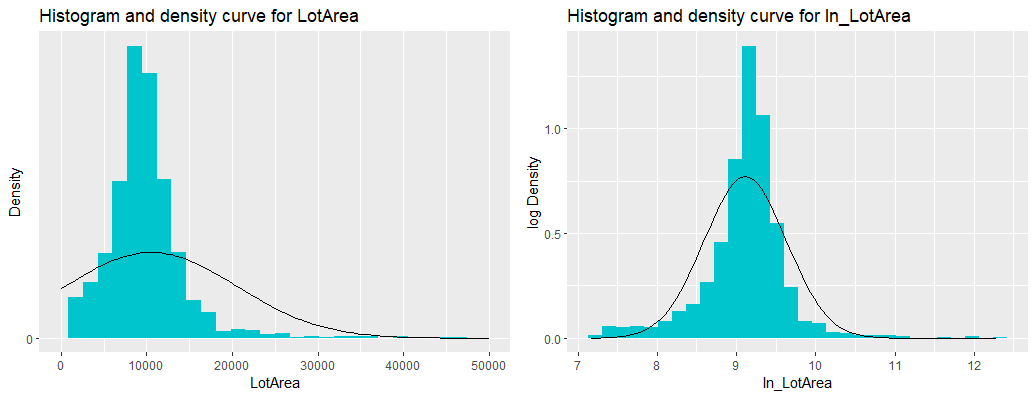
\includegraphics[width=0.6\textwidth]{log_transformations.png}
    \label{fig:logtransform}
\end{figure}

\hyperref[fig:logtransform]{Figure 9} takes a look at the distribution of \emph{LotArea}. Generally speaking, all quantitative variables in the baseline model are rather skewed and deviate from normality, but \emph{LotArea} is picked for log transformation. \hyperref[fig:logtransform]{Figure 9} shows the variable before and after the functional log transformation to swing it toward normality. Much improvement toward normal distribution can be observed.

\begin{table}[!htbp]
\centering
\caption{\label{tab:SWtest} Results of the Shapiro-Wilk test on the variables of baseline model.}
\begin{tabular}{l|r|r}
\hline
  & SW\_test\_statistic & SW\_p\_value\\
\hline
LotArea & 0.3510589 & 0.0000000\\
\hline
ln\_LotArea & 0.9054287 & 0.0000000\\
\hline
GarageArea & 0.9753273 & 0.0000000\\
\hline
OverallQual & 0.9480078 & 0.0000000\\
\hline
\end{tabular}
\end{table}

Normality of the regressors can be assessed by performing Shapiro-Wilk test for normality. The null hypothesis conforms with normal distribution, while the rejection with the lack of normal distribution. \hyperref[tab:SWtest]{Table 7} showcases the results. None of the variables are distributed normally according to the S-W test as test statistics yield significant results at a p-value lower than 0.00000001. However, worth noting here are the shortcomings of this procedure. It's possible to prove that when sample size gets large, even the smallest deviations from normality will lead to a significant result of Shapiro-Wilk test. And as every dataset has some degree of randomness, no single dataset will be a perfectly normally distributed sample. In that case, for the sake of this reporting that deals with large sample, the results of this test are not pertinent to the analysis.

\section{Subset analyses}

In this section the baseline model developed in preceding sections of the document will be scrutinized using sub-sample analyses based on the available dataset.

\subsection{Baseline model adjusted for the sub-sample of AC units}

What is undoubtedly of high value to stakeholders on the housing market in \href{https://www.google.com/maps/place/Ames,+IA,+USA/@42.0258192,-93.6964165,12z/data=!4m13!1m7!3m6!1s0x87ee70624634a06b:0x273156083cc75200!2sAmes,+IA,+USA!3b1!8m2!3d42.0307812!4d-93.6319131!3m4!1s0x87ee70624634a06b:0x273156083cc75200!8m2!3d42.0307812!4d-93.6319131}{Ames, Iowa} is the availability of AC units. Given a drastic change in average temperatures across seasons (average in summer +30Celsius, average in winter -3Celsius) it is a desired amenity. This fact is reflected in the dataset as there is an overwhelming amount of houses with AC against those that do not have it. 

Nonetheless, the baseline model is being fit for a sub-sample of both houses without AC (1) and with AC (2) and that is compared with a baseline model (3) in the \hyperref[tab:acunits]{Table 8}.

\begin{table}[h]
\centering
\caption{\label{tab:acunits} Sub-sampling the data for an existence of AC against a baseline model.}
\begin{tabular}{@{\extracolsep{5pt}}lccc} 
\\[-1.8ex]\hline 
\hline \\[-1.8ex] 
 & \multicolumn{3}{c}{\textit{Dependent variable:}} \\ 
\cline{2-4} 
\\[-1.8ex] & \multicolumn{3}{c}{SalePrice} \\ 
\\[-1.8ex] & (1) & (2) & (3)\\ 
\hline \\[-1.8ex] 
 LotArea & 2.869$^{***}$ & 1.092$^{***}$ & 1.112$^{***}$ \\ 
  & (0.774) & (0.120) & (0.118) \\ 
  & & & \\ 
 GarageArea & 43.657$^{***}$ & 85.862$^{***}$ & 85.709$^{***}$ \\ 
  & (13.506) & (6.951) & (6.527) \\ 
  & & & \\ 
 dLotShapeRegular0 & 11,424.840 & 11,485.520$^{***}$ & 11,916.440$^{***}$ \\ 
  & (7,775.110) & (2,532.650) & (2,467.157) \\ 
  & & & \\ 
 OverallQual & 15,961.680$^{***}$ & 37,620.940$^{***}$ & 36,311.880$^{***}$ \\ 
  & (2,211.885) & (1,074.735) & (1,005.548) \\ 
  & & & \\ 
 Constant & $-$8,403.656 & $-$104,743.400$^{***}$ & $-$97,156.920$^{***}$ \\ 
  & (11,647.510) & (5,699.414) & (5,229.643) \\ 
  & & & \\ 
\hline \\[-1.8ex] 
Observations & 95 & 1,365 & 1,460 \\ 
R$^{2}$ & 0.577 & 0.693 & 0.700 \\ 
Adjusted R$^{2}$ & 0.558 & 0.692 & 0.699 \\ 
Residual Std. Error & 27,046.040 (df = 90) & 43,756.710 (df = 1360) & 43,569.400 (df = 1455) \\ 
F Statistic & 30.642$^{***}$ (df = 4; 90) & 766.050$^{***}$ (df = 4; 1360) & 848.907$^{***}$ (df = 4; 1455) \\ 
\hline 
\hline \\[-1.8ex] 
\textit{Note:}  & \multicolumn{3}{r}{$^{*}$p$<$0.1; $^{**}$p$<$0.05; $^{***}$p$<$0.01} \\ 
\end{tabular} 
\end{table} 

Evidently, the estimates swing away from the baseline model's estimations for the model without the AC. It is mostly prompted by the disproportion of observations in terms of having the AC or not. Only 95 observations are without AC units, which makes the model a bit worse in terms of the goodness-of-fit and accelerates calculations of standard errors. Also as a consequence of the disproportion of the observations, the model accounting for existence of AC in the houses is very close to the baseline model. The sub-sampling procedure for AC units yields results that are not very informative and are rather due to technicalities behind the OLS technique.

\subsection{Baseline model adjusted for the sub-sample of age of the house}

Given dataset does not provide an age of the house directly, but it can be derived from the year in which the house was build as well as the year of a remodelling (if occured). This manipulation results in a prospect of investigating whether the age of the house impacts the baseline model and in what way. The expectation would be that newer houses will have a nominally higher coefficients and that the sale price is associated negatively with the age.

\begin{table}[h]
\centering
\caption{\label{tab:age} Sub-sampling the age of the house against a baseline model.}
\begin{tabular}{@{\extracolsep{5pt}}lcc} 
\\[-1.8ex]\hline 
\hline \\[-1.8ex] 
 & \multicolumn{2}{c}{\textit{Dependent variable:}} \\ 
\cline{2-3} 
\\[-1.8ex] & \multicolumn{2}{c}{SalePrice} \\ 
\\[-1.8ex] & (1) & (2)\\ 
\hline \\[-1.8ex] 
 LotArea & 1.444$^{***}$ & 1.068$^{***}$ \\ 
  & (0.227) & (0.104) \\ 
  & & \\ 
 GarageArea & 85.715$^{***}$ & 62.728$^{***}$ \\ 
  & (11.713) & (6.200) \\ 
  & & \\ 
 dLotShapeRegular & $-$8,952.658$^{**}$ & $-$15,011.280$^{***}$ \\ 
  & (4,006.265) & (2,491.620) \\ 
  & & \\ 
 OverallQual & 39,791.650$^{***}$ & 25,712.200$^{***}$ \\ 
  & (1,878.406) & (1,084.306) \\ 
  & & \\ 
 Constant & $-$108,503.900$^{***}$ & $-$21,116.180$^{***}$ \\ 
  & (10,919.350) & (6,426.575) \\ 
  & & \\ 
\hline \\[-1.8ex] 
Observations & 732 & 728 \\ 
R$^{2}$ & 0.656 & 0.635 \\ 
Adjusted R$^{2}$ & 0.654 & 0.633 \\ 
Residual Std. Error & 51,290.870 (df = 727) & 30,078.790 (df = 723) \\ 
F Statistic & 347.074$^{***}$ (df = 4; 727) & 314.238$^{***}$ (df = 4; 723) \\ 
\hline 
\hline \\[-1.8ex] 
\textit{Note:}  & \multicolumn{2}{r}{$^{*}$p$<$0.1; $^{**}$p$<$0.05; $^{***}$p$<$0.01} \\ 
\end{tabular} 
\end{table} 

Rerunning the baseline model for the sub-sample of age follows the intuition. \hyperref[tab:age]{Table 9} shows that coefficients for newer houses (cut-off at the median age of 28) are of higher magnitude and indicate stronger association.

\begin{figure}[h]
    \caption{Sub-sampling for age against a baseline model}.
    \centering
    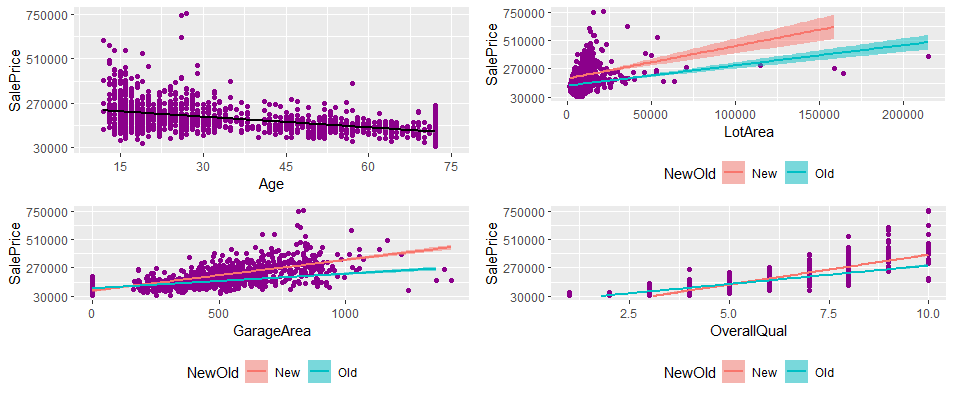
\includegraphics[width=0.6\textwidth]{age-subsample.png}
    \label{fig:agesubsample}
\end{figure}

\hyperref[fig:agesubsample]{The graphical evidence in Figure 10} points in the same direction overall (top-left figure) and per variable. Steeper lines for newer houses indicate higher coefficients and stronger linear relationship, while higher placement of the line in the scatter for new houses implicates higher prices for said units altogether. The sub-sampling procedure corroborated initial analytical thoughts and uncovered interesting relationship that might prove useful to the stakeholders 


\appendix

\section{Appendix - code}
\begin{tiny}
\begin{minted}{R}


############################################################################
############################################################################
###                                                                      ###
###                ALEKSANDER ODZIEMKOWSKI, BAM01 AS&P                   ###
###                INDIVIDUAL ASSIGNMENT 1, 16.09.2022                   ###
###                                                                      ###
############################################################################
############################################################################


##################################################################
##              Setting up the IDE and environment              ##
##################################################################

# ----------------------------------
# Clear the console and environment
# ----------------------------------
remove(list=ls())
cat("\f")

# ---------
# Packages
# ---------
library(bannerCommenter)
library(stargazer)
library(magrittr)
library(forcats)
library(olsrr)
library(corrplot)
library(lm.beta)
library(knitr)
library(plyr)
library(MASS)
library(gridExtra)
library(tidyverse)
library(sandwich)
library(car)

# ----------------------------------------------------
# Set working directory and define folder's structure
# ----------------------------------------------------
setwd("C:/STUDIA - materiały/RSM-MASTERS/COURSES/BLOCK 1/Advanced Statistics and Programming/Assignment 1")

dir <- "C:/STUDIA - materiały/RSM-MASTERS/COURSES/BLOCK 1/Advanced Statistics and Programming/Assignment 1/"

dirData <- paste0(dir, "Data/")
dirProg <- paste0(dir, "Programs/")
dirRslt <- paste0(dir, "Results/")

#################################################################
##              Import and inspect the train data              ##
#################################################################

# ----------------------------
# Import CSV data - train.csv
# ----------------------------

housingDataAll <- read.csv(file = paste0(dirData, "train.csv"), header = TRUE)

# Performing checks on the data to see whether it loaded correctly (that is - as expected)

head(housingDataAll)
tail(housingDataAll)
summary(housingDataAll$SalePrice)
str(housingDataAll$OverallQual10)

# Checking n/a per variable as linear regression model will not handle missing values;
# One must investigate the missing values and whether decision to drop them is reasonable;
# Otherwise, such variables cannot be considered for the model;
# Investigate the pattern of n/a;

dfMissingValues <- as.data.frame(colSums(is.na(housingDataAll)))
colnames(dfMissingValues) <- c("# Missing Values")
columnsNA <- as.data.frame(housingDataAll[, dfMissingValues[,1] != 0])

#################################################################
##              Variables of choice for the model              ##
#################################################################

# LotArea
# LotShape
# GarageArea
# OverallQual

##############################################################################
##  Plots to support the story and to have an initial look at associations  ##
##############################################################################

# 1) Investigating possible non-linear terms among quantitative variables
scatterLinearTestLotArea <- ggplot(housingDataAll, aes(LotArea, SalePrice))

scatterLinearTestLotArea + geom_point() + 
  geom_smooth(method = "lm", colour = "Red") + 
  labs(x = "LotArea", y = "SalePrice") +
  scale_x_continuous(limits = c(0, 30000)) +
  scale_y_continuous(limits = c(0, 755000), breaks = seq(30000, 755000, by = 120000))

scatterLinearTestLotArea + geom_point() + 
  geom_smooth() + 
  labs(x = "LotArea", y = "SalePrice") +
  scale_x_continuous(limits = c(0, 30000)) +
  scale_y_continuous(limits = c(0, 755000), breaks = seq(30000, 755000, by = 120000))

scatterLinearTestGarageArea <- ggplot(housingDataAll, aes(GarageArea, SalePrice))

scatterLinearTestGarageArea + geom_point() + 
  geom_smooth(method = "lm", colour = "Red") + 
  labs(x = "GarageArea", y = "SalePrice") +
  scale_x_continuous(limits = c(0, 1000)) +
  scale_y_continuous(limits = c(0, 755000), breaks = seq(30000, 755000, by = 120000))

scatterLinearTestGarageArea + geom_point() + 
  geom_smooth() + 
  labs(x = "GarageArea", y = "SalePrice") +
  scale_x_continuous(limits = c(0, 1000)) +
  scale_y_continuous(limits = c(0, 755000), breaks = seq(30000, 755000, by = 120000))

#  2) Possible interaction effect LotArea*LotShape against SalePrice
scatterLotShapeInteraction <- ggplot(data = housingDataAll, aes(x = LotArea, y = SalePrice, colour = LotShape))

scatterLotShapeInteraction +
  geom_point() +
  geom_smooth(method = 'lm', aes(fill=LotShape), alpha = 0.5) +
  labs(x = "LotArea", y = "SalePrice") +  
  theme(legend.position="bottom") +
  scale_y_continuous(limits = c(30000, 755000), breaks = seq(30000, 755000, by = 120000))

# 3) Bar chart with LotShape showing that merging irregular shapes is desired
barBaseShapeAggregate <- ggplot(data = housingDataAll, aes(x = fct_infreq(LotShape)))

barBaseShapeAggregate + 
  geom_bar(aes(fill = LotShape), stat = "count") +
  geom_text(aes(LotShape, label = signif((..count..)/sum(..count..), 2)), stat = "count", nudge_y = 30) +
  labs(x = "LotShape", y = "Count") +
  theme(legend.position="bottom") +
  scale_y_continuous(limits = c(0, 1000), breaks = seq(0, 1000, by = 250), name = "Count of instances of each lot shape", sec.axis = sec_axis(~ . / 1460, 
  name = "Ratio of instances of lot shape to total # of lots"))

# 4) Scatter plot with fitted line for GarageArea vs. SalePrice
scatterBaseGarageArea <- ggplot(data = housingDataAll, aes(x = GarageArea, y = SalePrice))

scatterBaseGarageArea +
  geom_point() +
  geom_smooth(method = 'lm', alpha = 0.5) +
  labs(x = "GarageArea", y = "SalePrice") +
  theme(legend.position="bottom") +
  scale_x_continuous(limits = c(0, 1500), breaks = seq(0, 1500, by = 300)) +
  scale_y_continuous(limits = c(30000, 755000), breaks = seq(30000, 755000, by = 120000))

# 5) Overall material and finish quality plotted against SalePrice
scatterBaseQualityLinear <- ggplot(data = housingDataAll, aes(x = OverallQual, y = SalePrice, colour = OverallQual))

scatterBaseQualityLinear +
  geom_point() +
  geom_smooth(method = 'lm', aes(fill=OverallQual), alpha = 0.5) +
  labs(x = "OverallQual", y = "SalePrice") +
  xlim(1, 10) +
  scale_x_continuous(breaks = seq(1, 10, by = 1)) +
  scale_y_continuous(limits = c(30000, 755000), breaks = seq(30000, 755000, by = 120000))

#  For saving the latest plot 
# ggsave(paste0(dirRslt, "scatterBaseQualityLinear.png"), width=8, height=6)

##################################################################
##           Data manipulation; dummy transformations           ##
##################################################################

# Reflection on whether the OverallQual has to remain categorical or can be expressed numerically in the model
#'What has to be done is the following:
#'Prepare a temporary object for a regression analysis: Id, SalePrice, OverallQual, dummies for OverallQual
#'Two regression models: SalePrice on OverallQual as discrete, SalePrice on OverallQual dummies
#'In dummy model - if there is a constant increase in coefficiants then it is an indication of linearity
#'In discrete model - does the coefficient hint at an rather steep positive effect of OverallQual on SalePrice? 

overallQual_lintest.df <-
  housingDataAll %>% 
  dplyr::select(Id, SalePrice, OverallQual)

# Necessary manipulation for dummies
overallQual_lintest.df$dOverallQual2 <- ifelse(overallQual_lintest.df$OverallQual == "2", 1, 0)
overallQual_lintest.df$dOverallQual3 <- ifelse(overallQual_lintest.df$OverallQual == "3", 1, 0)
overallQual_lintest.df$dOverallQual4 <- ifelse(overallQual_lintest.df$OverallQual == "4", 1, 0)
overallQual_lintest.df$dOverallQual5 <- ifelse(overallQual_lintest.df$OverallQual == "5", 1, 0)
overallQual_lintest.df$dOverallQual6 <- ifelse(overallQual_lintest.df$OverallQual == "6", 1, 0)
overallQual_lintest.df$dOverallQual7 <- ifelse(overallQual_lintest.df$OverallQual == "7", 1, 0)
overallQual_lintest.df$dOverallQual8 <- ifelse(overallQual_lintest.df$OverallQual == "8", 1, 0)
overallQual_lintest.df$dOverallQual9 <- ifelse(overallQual_lintest.df$OverallQual == "9", 1, 0)
overallQual_lintest.df$dOverallQual10 <- ifelse(overallQual_lintest.df$OverallQual == "10", 1, 0)

# Factoring dummies
overallQual_lintest.df$dOverallQual2 <- factor(overallQual_lintest.df$dOverallQual2, levels = c(0, 1))
overallQual_lintest.df$dOverallQual3 <- factor(overallQual_lintest.df$dOverallQual3, levels = c(0, 1))
overallQual_lintest.df$dOverallQual4 <- factor(overallQual_lintest.df$dOverallQual4, levels = c(0, 1))
overallQual_lintest.df$dOverallQual5 <- factor(overallQual_lintest.df$dOverallQual5, levels = c(0, 1))
overallQual_lintest.df$dOverallQual6 <- factor(overallQual_lintest.df$dOverallQual6, levels = c(0, 1))
overallQual_lintest.df$dOverallQual7 <- factor(overallQual_lintest.df$dOverallQual7, levels = c(0, 1))
overallQual_lintest.df$dOverallQual8 <- factor(overallQual_lintest.df$dOverallQual8, levels = c(0, 1))
overallQual_lintest.df$dOverallQual9 <- factor(overallQual_lintest.df$dOverallQual9, levels = c(0, 1))
overallQual_lintest.df$dOverallQual10 <- factor(overallQual_lintest.df$dOverallQual10, levels = c(0, 1))

# Fit the models
model_overallQual_lin_discrete <- lm(SalePrice ~ OverallQual, data = overallQual_lintest.df)
model_overallQual_lin_dummy <- lm(SalePrice ~ dOverallQual2 + dOverallQual3 + dOverallQual4 + dOverallQual5 + dOverallQual6 + dOverallQual7 + dOverallQual8 + dOverallQual9 + 
dOverallQual10, data = overallQual_lintest.df)

stargazer(model_overallQual_lin_discrete, model_overallQual_lin_dummy)

# Conclusion - we can work with OverallQual as a numerical variable instead of a scale (to be transformed to dummy) 
# because of the linear relationship of effects of consecutive increase in quality (seen in lm result and the graph). 
# The direct interpretation of beta will have no precise meaning, but the general association and standardized strength of the effect 
# can now be measured and interpreted more easily. 

# Dummy transformation
# Given a proportion of regular shaped homes to those irregularly shaped under IR1, IR2 and IR3 - group irregulars together
# Merging IR1, IR2, IR3 into IR
housingDataAll$LotShape <- ifelse(housingDataAll$LotShape == "Reg", "Regular", "Irregular")
housingDataAll$dLotShapeRegular <- ifelse(housingDataAll$LotShape == "Regular", "Regular", "Irregular")

# LotShape into dummy variable - 1 describes regular shape, 0 describes irregular shape
housingDataAll$dLotShapeRegular <- ifelse(housingDataAll$dLotShapeRegular == "Regular", 1, 0)

# Perform a check on the transformation
dplyr::select(housingDataAll, c("LotShape", "dLotShapeRegular"))

# Combine relevant variables into a df that is gonna be an input to model 
housingData <- 
  housingDataAll %>% 
  dplyr::select(Id, SalePrice, LotArea, GarageArea, OverallQual, LotShape, dLotShapeRegular)

############################################################
##      Summary statistics of variables in the model      ##
############################################################

stargazer(housingData, type = "text", summary.stat = c("n", "mean", "sd", "min", "p25", "median", "p75", "max"), omit = "Id", digits = 2)

# Latex
stargazer(housingData, summary.stat = c("mean", "sd", "min", "p25", "median", "p75", "max"), omit = "Id", digits = 2)

# Coefficient of variance
cov_results <- round(cbind(SalePriceCV = sd(housingData$SalePrice)/mean(housingData$SalePrice),
      LotAreaCV = sd(housingData$LotArea)/mean(housingData$LotArea),
      GarageAreaCV = sd(housingData$GarageArea)/mean(housingData$GarageArea),
      OverallQualCV = sd(housingData$OverallQual)/mean(housingData$OverallQual),
      dLotShapeRegularCV = sd(housingData$dLotShapeRegular)/mean(housingData$dLotShapeRegular)
), 4)

# --------
# Factors
# --------
# Categorical variables (LotShape and dLotShapeRegular) to factors
housingData$LotShape <- factor(housingData$LotShape, levels = c("Irregular", "Regular"))
housingData$dLotShapeRegular <- factor(housingData$dLotShapeRegular, levels = c(0, 1))

####################################################################
##  Drawing a causal relationship scheme and developing a theory  ##
####################################################################

# Done outside of the code

############################################################################
##      Formulating research hypotheses and population regression models  ##
############################################################################

# H1: Garage area has a positive influence on the sale price of the house.
# H2: The expected sale price of the house is higher for houses with a better overall material and finish of the house.
# H3: The positive influence of lot size on sale price of the house is expected to be larger for regularly shaped houses than for irregularly shaped houses.


# Should quadratic terms be introduced for quantitative variables in the model in terms of model fit? And for which?
# LotArea goodness-of-fit
linear_LotArea <- lm(SalePrice ~ LotArea, data = housingDataAll)
quadratic_LotArea <- lm(SalePrice ~ LotArea + I(LotArea^2), data = housingDataAll)
stargazer(linear_LotArea, quadratic_LotArea, type = 'text')

# GarageArea goodness-of-fit
linear_GarageArea <- lm(SalePrice ~ GarageArea, data = housingDataAll)
quadratic_GarageArea <- lm(SalePrice ~ GarageArea + I(GarageArea^2), data = housingDataAll)
stargazer(linear_GarageArea, quadratic_GarageArea, type = 'text')
# Conclusion : R2 improvement suggest that introducing quadratic terms for LotArea will improve the model fit better. 

# -----------------------------
# Population regression models
# -----------------------------
# Introduced outside of the code

##################################################################
##   Estimating the baseline model and further specifications   ##
##################################################################

model_baseline <- lm(SalePrice ~ LotArea + GarageArea + dLotShapeRegular + OverallQual, data = housingData)

model_interactions <- lm(SalePrice ~ LotArea + LotArea*dLotShapeRegular + GarageArea + dLotShapeRegular + OverallQual, data = housingData)

model_nonlinear <- lm(SalePrice ~ LotArea + I(LotArea^2) + GarageArea + dLotShapeRegular + OverallQual, data = housingData)

model_interactions_nonlinear <- lm(SalePrice ~ LotArea + I(LotArea^2) + LotArea*dLotShapeRegular + GarageArea + dLotShapeRegular + OverallQual, data = housingData)

stargazer(model_baseline, model_interactions, model_nonlinear, type = "text")

stargazer(model_interactions_nonlinear, type = "text")

##################################################################
##                     Standardized effects                     ##
##################################################################

# Calculate standardized effects
lm_baseline_beta <- lm.beta(model_baseline)
lm_interactions_beta <- lm.beta(model_interactions)
lm_nonlinear_beta <- lm.beta(model_nonlinear)
lm_interactions_nonlinear_beta <- lm.beta(model_interactions_nonlinear)

# Manipulation of results to arrive at a final df to be used for reporting

# Set up data frames for standardized coefficients
baselina_beta_df <- as.data.frame(lm_baseline_beta[["standardized.coefficients"]], col.names = names(c("Standardized coefficients")))
interactions_beta_df <- as.data.frame(lm_interactions_beta[["standardized.coefficients"]], col.names = names(c("Standardized coefficients")))
nonlinear_beta_df <- as.data.frame(lm_nonlinear_beta[["standardized.coefficients"]], col.names = names(c("Standardized coefficients")))
interactions_nonlinear_beta_df <- as.data.frame(lm_interactions_nonlinear_beta[["standardized.coefficients"]], col.names = names(c("Standardized coefficients")))

# First generate original data.frames
building_stand_coeff1 <- merge(baselina_beta_df, interactions_beta_df, by = 0, all = TRUE)
building_stand_coeff2 <- merge(nonlinear_beta_df, interactions_nonlinear_beta_df, by = 0, all = TRUE)

# Then use first column for row names
building_stand_coeff1 <- data.frame(building_stand_coeff1, row.names = 1)
building_stand_coeff2 <- data.frame(building_stand_coeff2, row.names = 1)

# Merge again 
standardized_coefficients <- merge(building_stand_coeff1, building_stand_coeff2, by = 0, all = TRUE)

# Use first column for row names and change remaining columns' names to arrive at a final df
standardized_coefficients <- data.frame(standardized_coefficients, row.names = 1)
colnames(standardized_coefficients) <- c("Baseline", "Interactions", "Non-linear", "Interactions and non-linear")

# Output 
kable(round(standardized_coefficients, 4), "latex")

#################################################################
##         Diagnostic analyses of the estimated models         ##
#################################################################

# -----------------------------------
# Normality of independent variables
# -----------------------------------
#LotArea
lotarea_hist <- ggplot(data = housingData, aes(x = LotArea))
bp <- lotarea_hist + 
  geom_histogram(aes(y = ..density..), fill = "turquoise3") + 
  labs(x = "LotArea", y = "Density") + 
  scale_x_continuous(limits = c(0, 50000)) +
  scale_y_continuous(breaks = seq(0, 0.2, by = 0.005)) +
  stat_function(
    fun = dnorm, 
    args = with(housingData, c(mean = mean(LotArea), sd = sd(LotArea)))) +
  ggtitle("Histogram and density curve for LotArea")

#GarageArea
garagearea_hist <- ggplot(data = housingData, aes(x = GarageArea))
dp <- garagearea_hist + 
  geom_histogram(aes(y = ..density..), fill = "turquoise3") + 
  labs(x = "GarageArea", y = "Density") + 
  scale_y_continuous(breaks = seq(0, 0.2, by = 0.005)) +
  stat_function(
    fun = dnorm, 
    args = with(housingData, c(mean = mean(GarageArea), sd = sd(GarageArea)))) +
  ggtitle("Histogram and density curve for GarageArea")

# OverallQual
overallqual_hist <- ggplot(data = housingData, aes(x = OverallQual))
vp <- overallqual_hist + 
  geom_histogram(aes(y = ..density..), fill = "turquoise3") + 
  labs(x = "OverallQual", y = "Density") + 
  stat_function(
    fun = dnorm, 
    args = with(housingData, c(mean = mean(OverallQual), sd = sd(OverallQual)))) +
  ggtitle("Histogram and density curve for OverallQual")

# Remedy for the non-normality of LotArea - log transformation
housingData$ln_LotArea <- log(housingData$LotArea)
ln_lotarea_hist <- ggplot(data = housingData, aes(x = ln_LotArea))
sc <- ln_lotarea_hist + 
  geom_histogram(aes(y = ..density..), fill = "turquoise3") + 
  labs(x = "ln_LotArea", y = "log Density") + 
  stat_function(
    fun = dnorm, 
    args = with(housingData, c(mean = mean(ln_LotArea), sd = sd(ln_LotArea)))) +
  ggtitle("Histogram and density curve for ln_LotArea")

# Combine graphs with gridExtra
grid.arrange(bp, sc, ncol=2, nrow =1)

# Shapiro-Wilk test - aggregation for the reporting
shap_lotarea <- shapiro.test(housingData$LotArea)
shap_garagearea <- shapiro.test(housingData$GarageArea)
shap_overallqual <- shapiro.test(housingData$OverallQual)
shap_ln_lotarea <- shapiro.test(housingData$ln_LotArea)

var_name <- c("LotArea", "ln_LotArea", "GarageArea", "OverallQual")
SW_test_statistic <- c(shap_lotarea[["statistic"]], shap_ln_lotarea[["statistic"]], shap_garagearea[["statistic"]], shap_overallqual[["statistic"]])
SW_p_value <- c(shap_lotarea[["p.value"]], shap_ln_lotarea[["p.value"]], shap_garagearea[["p.value"]], shap_overallqual[["p.value"]])

shapiro_results <- data.frame(var_name,
                              SW_test_statistic,
                              SW_p_value,
                              row.names = var_name)

shapiro_results <-
  shapiro_results %>%
  dplyr::select(SW_test_statistic, SW_p_value)

kable(shapiro_results, "latex")

# Run simple regression model with LotArea and lnLotArea
model_lotarea_norm <- lm(SalePrice ~ LotArea, data = housingData)
model_ln_lotarea_norm <- lm(SalePrice ~ ln_LotArea, data = housingData)

stargazer(model_lotarea_norm, model_ln_lotarea_norm, type = 'text')

# -----------------------------------
# Homoscedasticity of the error term
# -----------------------------------

# Plot Residuals vs. Fitted for graphical evidence

# par(mfrow=c(1,2))
ols_plot_resid_fit(model_baseline)
ols_plot_resid_fit(model_interactions_nonlinear)
# par(mfrow=c(1,1))

# Perform Breusch-Pagan test for test-based evidence
lmtest::bptest(model_baseline)
lmtest::bptest(model_interactions_nonlinear)

# Remedy for heteroscedasticity - robust standard errors (they are more conservative)
seBasic <- sqrt(diag(vcov(model_baseline)))
seWhite <- sqrt(diag(vcovHC(model_baseline, type = 'HC0')))
seClust <- sqrt(diag(vcovHC(model_baseline, cluster = 'dLotShapeRegular')))

stargazer(model_baseline, model_baseline, model_baseline, se = list(seBasic, seWhite, seClust), type = 'text')

# -------------------------------
# Is multicollinearity a problem?
# -------------------------------

# Using VIF to assess whether multicollinearity exists in the model

vif_base <- vif(model_baseline)

stargazer(vif_base, type = 'text')

# There are no objective threshold, but vif = 5 may be used as a proxy for an existence of multicollinearity in the data

# Correlation matrix
subset_cor <- 
  housingData %>%
  select(SalePrice, LotArea, GarageArea, OverallQual)

corrplot(cor(subset_cor), method = "number")

# Remedy for multicollinearity - problem non-existent in the model

# -----------------------------------------------------------------------------------
# Analyzing the (standardized) residuals to assess whether their behavior is consistent 
# with the assumptions of the linear regression model
# -----------------------------------------------------------------------------------

# Inspecting residuals
resids_baseline <- residuals(model_baseline)
resids_interactions <- residuals(model_interactions)
resids_nonlinear <- residuals(model_nonlinear)
resids_interactions_nonlinear <- residuals(model_interactions_nonlinear)

residuals <- data.frame(resids_baseline, resids_interactions, resids_nonlinear, resids_interactions_nonlinear)

# Inspecting studentized residuals
studresids_baseline <- studres(model_baseline)
studresids_interactions <- studres(model_interactions)
studresids_nonlinear <- studres(model_nonlinear)
studresids_interactions_nonlinear <- studres(model_interactions_nonlinear)

stud_residuals <- data.frame(studresids_baseline, studresids_interactions, studresids_nonlinear, studresids_interactions_nonlinear)

# if the assumption of OLS holds, we should see 0 as the mean (it is an empirical mean, can be NOT EXACTLY 0, like -0)
# also looking at the range, we want residuals to be normally distribute, so the min-max should be of same magnitute
stargazer(residuals, stud_residuals, type = 'text')

# Residual vs Fitted Values Plot
#par(mfrow=c(2,2))
plot(fitted(model_baseline), resids_baseline, abline(0,0), main="Residuals vs Fitted Baseline")
plot(fitted(model_interactions), resids_interactions, abline(0,0), main="Residuals vs Fitted Interactions")
plot(fitted(model_nonlinear), resids_nonlinear, abline(0,0), main="Residuals vs Fitted Nonlinear")
plot(fitted(model_interactions_nonlinear), resids_interactions_nonlinear, abline(0,0), main="Residuals vs Fitted Interactions and Nonlinear")
#par(mfrow=c(1,1))

# Studentized Residual vs Fitted Values Plot
# par(mfrow=c(2,2))
plot(fitted(model_baseline), studresids_baseline, abline(0,0), main="Stu_Residuals vs Fitted Baseline")
plot(fitted(model_interactions), studresids_interactions, abline(0,0), main="Stu_Residuals vs Fitted Interactions")
plot(fitted(model_nonlinear), studresids_nonlinear, abline(0,0), main="Stu_Residuals vs Fitted Nonlinear")
plot(fitted(model_interactions_nonlinear), studresids_interactions_nonlinear, abline(0,0), main="Stu_Residuals vs Fitted Interactions and Nonlinear")
# par(mfrow=c(1,1))

#################################################################
##                       Subset analyses                       ##
#################################################################

# ---------------------------------------------
# Does the model differ for AC unit in houses?
# ---------------------------------------------

# Familiarize with the data
table(housingDataAll$CentralAir)
joinAC <- housingDataAll %>%
  dplyr::select(Id, CentralAir)

# Adjust housingData and run the models
housingDataAC <- merge(housingData, joinAC, by = "Id")
housingDataAC_N <- subset(housingDataAC, CentralAir == "N")
housingDataAC_Y <- subset(housingDataAC, CentralAir == "Y")
submodel_AC_N <- lm(SalePrice ~ LotArea + GarageArea + dLotShapeRegular + OverallQual, data = housingDataAC_N)
submodel_AC_Y <- lm(SalePrice ~ LotArea + GarageArea + dLotShapeRegular + OverallQual, data = housingDataAC_Y)

stargazer(submodel_AC_N, submodel_AC_Y, type = 'text')

# ---------------------------------------------------------------------------------------------
# Does the Age (YearRemodAdd - YearBuilt) affect the SalePrice and other effects in the model?
# ---------------------------------------------------------------------------------------------

# Set up new df with special variable "Age"
housingDataAge <- 
  housingDataAll %>%
  dplyr::select(Id, SalePrice, LotArea, GarageArea, OverallQual, LotShape, dLotShapeRegular, YearRemodAdd, YearBuilt)

housingDataAge$Age <- case_when(
  housingDataAge$YearRemodAdd == housingDataAge$YearBuilt ~ as.integer(format(Sys.Date(), "%Y")) - housingDataAge$YearBuilt,
  housingDataAge$YearRemodAdd != housingDataAge$YearBuilt ~ as.integer(format(Sys.Date(), "%Y")) - housingDataAge$YearRemodAdd
)

# Inspection of the Age distribution
age_histogram <- ggplot(data = housingDataAge, aes(Age))
age_histogram + geom_histogram(binwidth = 5) + labs(x = "Age", y = "Frequency")

#Splitting houses into "New" and "Old" based on the median of the Age (28)
median(housingDataAge$Age)

housingDataAge$NewOld <- if_else(housingDataAge$Age > 28, "Old", "New")
# table(housingDataAge$NewOld) 728 732

#Subset of New and Old for the model
housingDataAgeNew <- subset(housingDataAge, NewOld == "New")
housingDataAgeOld <- subset(housingDataAge, NewOld == "Old")

# Build a model and compare results
submodel_age_new <- lm(SalePrice ~ LotArea + GarageArea + dLotShapeRegular + OverallQual, data = housingDataAgeNew)
submodel_age_old <- lm(SalePrice ~ LotArea + GarageArea + dLotShapeRegular + OverallQual, data = housingDataAgeOld)

stargazer(submodel_age_new, submodel_age_old, type = 'text')

# Graphical evidence for the models' results
ad <- 
  ggplot(data = housingDataAge, aes(x = Age, y = SalePrice)) +
  geom_point(colour = "magenta4") +
  geom_smooth(method = 'lm', alpha = 0.5, colour = "black") +
  labs(x = "Age", y = "SalePrice") +
  theme(legend.position="bottom") +
  scale_x_continuous(limits = c(10, 75), breaks = seq(0, 75, by = 15)) +
  scale_y_continuous(limits = c(30000, 755000), breaks = seq(30000, 755000, by = 240000))

ko <- 
  ggplot(data = housingDataAge, aes(x = LotArea, y = SalePrice, colour = NewOld)) +
  geom_point(colour = "magenta4") +
  geom_smooth(method = 'lm', aes(fill=NewOld), alpha = 0.5) +
  labs(x = "LotArea", y = "SalePrice") +  
  theme(legend.position="bottom") +
  scale_y_continuous(limits = c(30000, 755000), breaks = seq(30000, 755000, by = 240000))

nl <- 
  ggplot(data = housingDataAge, aes(x = GarageArea, y = SalePrice, colour = NewOld)) +
  geom_point(colour = "magenta4") +
  geom_smooth(method = 'lm', aes(fill=NewOld), alpha = 0.5) +
  labs(x = "GarageArea", y = "SalePrice") +  
  theme(legend.position="bottom") +
  scale_y_continuous(limits = c(30000, 755000), breaks = seq(30000, 755000, by = 240000))

rt <-
  ggplot(data = housingDataAge, aes(x = OverallQual, y = SalePrice, colour = NewOld)) +
  geom_point(colour = "magenta4") +
  geom_smooth(method = 'lm', aes(fill=NewOld), alpha = 0.5) +
  labs(x = "OverallQual", y = "SalePrice") +  
  theme(legend.position="bottom") +
  scale_y_continuous(limits = c(30000, 755000), breaks = seq(30000, 755000, by = 240000))

# Combine graphs with gridExtra
grid.arrange(ad, ko, nl, rt, ncol=2, nrow =2)
\end{minted}
\end{tiny}

\section{Appendix - tables and figures}
\begin{table}[t]
\centering
\caption{\label{tab:overallqualldummy} Using \emph{OverallQual} as a numerical variable due to a good proxy to dummy variable's effects.}
\begin{tabular}{@{\extracolsep{5pt}}lcc} 
\\[-1.8ex]\hline 
\hline \\[-1.8ex] 
 & \multicolumn{2}{c}{\textit{Dependent variable:}} \\ 
\cline{2-3} 
\\[-1.8ex] & \multicolumn{2}{c}{SalePrice} \\ 
\\[-1.8ex] & (1) & (2)\\ 
\hline \\[-1.8ex] 
 OverallQual & 45,435.800$^{***}$ &  \\ 
  & (920.430) &  \\ 
  & & \\ 
 dOverallQual21 &  & 1,620.333 \\ 
  &  & (40,881.320) \\ 
  & & \\ 
 dOverallQual31 &  & 37,323.750 \\ 
  &  & (33,212.140) \\ 
  & & \\ 
 dOverallQual41 &  & 58,270.650$^{*}$ \\ 
  &  & (31,938.350) \\ 
  & & \\ 
 dOverallQual51 &  & 83,373.350$^{***}$ \\ 
  &  & (31,746.200) \\ 
  & & \\ 
 dOverallQual61 &  & 111,453.000$^{***}$ \\ 
  &  & (31,751.090) \\ 
  & & \\ 
 dOverallQual71 &  & 157,566.400$^{***}$ \\ 
  &  & (31,765.640) \\ 
  & & \\ 
 dOverallQual81 &  & 224,585.500$^{***}$ \\ 
  &  & (31,854.470) \\ 
  & & \\ 
 dOverallQual91 &  & 317,363.000$^{***}$ \\ 
  &  & (32,394.590) \\ 
  & & \\ 
 dOverallQual101 &  & 388,438.400$^{***}$ \\ 
  &  & (33,379.460) \\ 
  & & \\ 
 Constant & $-$96,206.080$^{***}$ & 50,150.000 \\ 
  & (5,756.407) & (31,666.530) \\ 
  & & \\ 
\hline \\[-1.8ex] 
Observations & 1,460 & 1,460 \\ 
R$^{2}$ & 0.626 & 0.684 \\ 
Adjusted R$^{2}$ & 0.625 & 0.682 \\ 
Residual Std. Error & 48,622.760 (df = 1458) & 44,783.240 (df = 1450) \\ 
F Statistic & 2,436.771$^{***}$ (df = 1; 1458) & 349.027$^{***}$ (df = 9; 1450) \\ 
\hline 
\hline \\[-1.8ex] 
\textit{Note:}  & \multicolumn{2}{r}{$^{*}$p$<$0.1; $^{**}$p$<$0.05; $^{***}$p$<$0.01} \\ 
\end{tabular} 
\end{table}

\begin{table}[t]
\centering
\caption{\label{tab:quadraticlotarea} Introduction of quadratic term to \emph{LotArea} resulting in relatively significant improvement in R2.}
\begin{tabular}{@{\extracolsep{5pt}}lcc} 
\\[-1.8ex]\hline 
\hline \\[-1.8ex] 
 & \multicolumn{2}{c}{\textit{Dependent variable:}} \\ 
\cline{2-3} 
\\[-1.8ex] & \multicolumn{2}{c}{SalePrice} \\ 
\\[-1.8ex] & (1) & (2)\\ 
\hline \\[-1.8ex] 
 LotArea & 2.100$^{***}$ & 6.029$^{***}$ \\ 
  & (0.201) & (0.419) \\ 
  & & \\ 
 I(LotArea$\hat{\mkern6mu}$2) &  & $-$0.00003$^{***}$ \\ 
  &  & (0.00000) \\ 
  & & \\ 
 Constant & 158,836.200$^{***}$ & 123,300.900$^{***}$ \\ 
  & (2,914.717) & (4,376.500) \\ 
  & & \\ 
\hline \\[-1.8ex] 
Observations & 1,460 & 1,460 \\ 
R$^{2}$ & 0.070 & 0.136 \\ 
Adjusted R$^{2}$ & 0.069 & 0.135 \\ 
Residual Std. Error & 76,653.770 (df = 1458) & 73,889.140 (df = 1457) \\ 
F Statistic & 109.090$^{***}$ (df = 1; 1458) & 114.776$^{***}$ (df = 2; 1457) \\ 
\hline 
\hline \\[-1.8ex] 
\textit{Note:}  & \multicolumn{2}{r}{$^{*}$p$<$0.1; $^{**}$p$<$0.05; $^{***}$p$<$0.01} \\ 
\end{tabular} 
\end{table} 

\begin{table}[t]
\centering
\caption{\label{tab:quadraticgaragearea} Introduction of quadratic term to \emph{GarageArea} resulting in not much of an improvement in terms of model fit.}
\begin{tabular}{@{\extracolsep{5pt}}lcc} 
\\[-1.8ex]\hline 
\hline \\[-1.8ex] 
 & \multicolumn{2}{c}{\textit{Dependent variable:}} \\ 
\cline{2-3} 
\\[-1.8ex] & \multicolumn{2}{c}{SalePrice} \\ 
\\[-1.8ex] & (1) & (2)\\ 
\hline \\[-1.8ex] 
 GarageArea & 231.646$^{***}$ & 169.510$^{***}$ \\ 
  & (7.608) & (21.954) \\ 
  & & \\ 
 I(GarageArea$\hat{\mkern6mu}$2) &  & 0.063$^{***}$ \\ 
  &  & (0.021) \\ 
  & & \\ 
 Constant & 71,357.420$^{***}$ & 83,742.000$^{***}$ \\ 
  & (3,949.003) & (5,689.315) \\ 
  & & \\ 
\hline \\[-1.8ex] 
Observations & 1,460 & 1,460 \\ 
R$^{2}$ & 0.389 & 0.392 \\ 
Adjusted R$^{2}$ & 0.388 & 0.392 \\ 
Residual Std. Error & 62,135.640 (df = 1458) & 61,963.820 (df = 1457) \\ 
F Statistic & 926.951$^{***}$ (df = 1; 1458) & 470.598$^{***}$ (df = 2; 1457) \\ 
\hline 
\hline \\[-1.8ex] 
\textit{Note:}  & \multicolumn{2}{r}{$^{*}$p$<$0.1; $^{**}$p$<$0.05; $^{***}$p$<$0.01} \\ 
\end{tabular} 
\end{table} 

\begin{table}[t]
\centering
\caption{\label{tab:sampleregressionall} Estimation of a sample regression model taking into account interaction and quadratic term.}
\begin{tabular}{@{\extracolsep{5pt}}lc} 
\\[-1.8ex]\hline 
\hline \\[-1.8ex] 
 & \multicolumn{1}{c}{\textit{Dependent variable:}} \\ 
\cline{2-2} 
\\[-1.8ex] & SalePrice \\ 
\hline \\[-1.8ex] 
 LotArea & 2.472$^{***}$ \\ 
  & (0.323) \\ 
  & \\ 
 I(LotArea$\hat{\mkern6mu}$2) & $-$0.00001$^{***}$ \\ 
  & (0.00000) \\ 
  & \\ 
 dLotShapeRegular1 & $-$15,621.220$^{***}$ \\ 
  & (5,283.637) \\ 
  & \\ 
 GarageArea & 74.980$^{***}$ \\ 
  & (6.622) \\ 
  & \\ 
 OverallQual & 36,523.610$^{***}$ \\ 
  & (990.998) \\ 
  & \\ 
 LotArea:dLotShapeRegular1 & 0.684 \\ 
  & (0.463) \\ 
  & \\ 
 Constant & $-$95,256.220$^{***}$ \\ 
  & (6,486.554) \\ 
  & \\ 
\hline \\[-1.8ex] 
Observations & 1,460 \\ 
R$^{2}$ & 0.710 \\ 
Adjusted R$^{2}$ & 0.709 \\ 
Residual Std. Error & 42,867.480 (df = 1453) \\ 
F Statistic & 592.963$^{***}$ (df = 6; 1453) \\ 
\hline 
\hline \\[-1.8ex] 
\textit{Note:}  & \multicolumn{1}{r}{$^{*}$p$<$0.1; $^{**}$p$<$0.05; $^{***}$p$<$0.01} \\ 
\end{tabular} 
\end{table}

\end{document}
